\documentclass[11pt,a4paper]{article}

\usepackage[margin=1in]{geometry}
% ---------------------------------------------------------------------------
% Shared preamble: packages, theorem environments, notation macros, and the
% listings style for delhi source.
% ---------------------------------------------------------------------------
\usepackage[T1]{fontenc}
\usepackage[utf8]{inputenc}
\usepackage[english]{babel}
\usepackage{lmodern}
\usepackage{microtype}

\usepackage{amsmath, amssymb, amsthm}
\usepackage{mathtools}
\usepackage{booktabs}
\usepackage{array}
\usepackage{listings}
\usepackage{xcolor}
\usepackage{tikz}
\usetikzlibrary{arrows.meta, positioning, fit, backgrounds, calc, shapes.geometric}
\usepackage[round,authoryear]{natbib}

% --- model-diagram styles --------------------------------------------------
% Worlds are circles labelled with the atoms true in them; the designated world
% carries a double ring. Plausibility edges point toward the *more* plausible world.
\tikzset{
  world/.style        = {circle, draw, minimum size=9.5mm, inner sep=1pt, font=\small},
  actual/.style       = {world, double, double distance=0.6pt},
  event/.style        = {rectangle, rounded corners=2pt, draw, minimum height=7mm,
                         minimum width=11mm, inner sep=2pt, font=\small},
  plaus/.style        = {-{Stealth[length=2mm]}, shorten >=1pt, shorten <=1pt},
  equi/.style         = {{Stealth[length=2mm]}-{Stealth[length=2mm]}, shorten >=1pt,
                         shorten <=1pt},
  elab/.style         = {font=\scriptsize, inner sep=1.5pt, fill=white},
  wlab/.style         = {font=\scriptsize\itshape, inner sep=1pt},
}
\usepackage[hidelinks]{hyperref}
\usepackage{cleveref}

% --- theorem environments --------------------------------------------------
% All theorem-like environments share one numbering sequence, so a reader meets
% Definition 2.1, Proposition 2.2, Theorem 2.3 rather than three interleaved series.
%
% The obvious way to do that -- \newtheorem{proposition}[definition]{Proposition} -- makes
% every environment literally use the counter named `definition`, and cleveref names a
% reference after its counter. The result is that \Cref of a proposition renders
% "Definition 2.5". `aliascnt` gives each environment a distinct counter name that is an
% alias for the same underlying counter, which keeps the shared sequence and lets cleveref
% tell them apart.
% All theorem-like environments share the `definition` counter, so a reader meets
% Definition 2.1, Proposition 2.2, Theorem 2.3 in one sequence.
%
% A consequence: cleveref names a reference after its *counter*, so \Cref of a
% proposition would render "Definition 2.5". The `aliascnt` package is the usual remedy,
% but it sends this document into an unterminating loop during AMS symbol-font setup.
% Cross-references to non-definition environments are therefore written explicitly --
% "Proposition~\ref{...}" rather than "\Cref{...}" -- and \cref is reserved for
% definitions, sections, tables and equations, where it names them correctly.
\theoremstyle{definition}
\newtheorem{definition}{Definition}[section]
\newtheorem{example}[definition]{Example}
\newtheorem{remark}[definition]{Remark}

\theoremstyle{plain}
\newtheorem{proposition}[definition]{Proposition}
\newtheorem{theorem}[definition]{Theorem}
\newtheorem{lemma}[definition]{Lemma}
\newtheorem{corollary}[definition]{Corollary}

% --- notation --------------------------------------------------------------
% Modalities are written with an explicit agent subscript throughout.
\newcommand{\Ag}{\mathcal{G}}                  % set of agents
\newcommand{\Props}{\mathcal{P}}               % set of propositions
\newcommand{\Worlds}{W}
\newcommand{\Kop}[1]{K_{#1}}                   % knowledge
\newcommand{\Bop}[1]{B_{#1}}                   % belief
\newcommand{\Sop}[1]{\Box_{#1}}                % safe belief
\newcommand{\Cop}[1]{C_{#1}}                   % common knowledge
\newcommand{\CBop}[2]{B^{#2}_{#1}}             % conditional belief
\newcommand{\Kw}[1]{\mathit{Kw}_{#1}}
\newcommand{\Bw}[1]{\mathit{Bw}_{#1}}
\newcommand{\Ig}[1]{\mathord{?}_{#1}}          % ignorance
\newcommand{\Susp}[1]{\mathord{\text{\textquestiondown}}_{#1}}

\newcommand{\plaus}[1]{R_{#1}}                 % plausibility preorder
\newcommand{\comp}[1]{\sim_{#1}}               % comparability
\newcommand{\best}[1]{\rightarrow_{#1}}        % maxima operator
\newcommand{\Lang}{\mathcal{L}}
\newcommand{\Lgb}{\Lang^{\Props}_{\Ag}}        % full modal language
\newcommand{\Lprop}{\Lang^{\Props}}            % propositional fragment
% Semantic brackets, defined here rather than via stmaryrd so the paper builds on a
% minimal TeX installation.
\providecommand{\llbracket}{[\![}
\providecommand{\rrbracket}{]\!]}
\newcommand{\denote}[1]{\llbracket #1 \rrbracket}
\newcommand{\bisimR}{\mathbin{\underline{\leftrightarrow}_{R}}}
\newcommand{\bisimD}{\mathbin{\underline{\leftrightarrow}_{D}}}
\newcommand{\ML}{\mathit{ML}}
\newcommand{\pre}{\mathit{pre}}
\newcommand{\add}{\mathit{add}}
\newcommand{\del}{\mathit{del}}
\newcommand{\FPN}{\mathit{FPN}}
\newcommand{\PN}{\mathit{PN}}
\newcommand{\Nlab}{\mathit{N}}
\newcommand{\hole}{\underline{\phantom{x}}}

% --- listings style for delhi source ---------------------------------------
\definecolor{kwcolor}{HTML}{6A3D9A}
\definecolor{clcolor}{HTML}{B15928}
\definecolor{cmcolor}{HTML}{6B7280}
\definecolor{opcolor}{HTML}{1F78B4}
\definecolor{bgcolor}{HTML}{F7F7F9}

\lstdefinelanguage{delhi}{
  morekeywords={types,objects,agents,props,constants,define,rules,initially,
                state,goal,invariants,actions},
  morekeywords=[2]{actor,pre,causes,determines,announces,observes,aware,if},
  morekeywords=[3]{K,B,C,Kw,Bw},
  sensitive=true,
  morecomment=[l]{//},
  morecomment=[s]{/*}{*/},
  morestring=[b]",
}

\lstset{
  language=delhi,
  basicstyle=\ttfamily\small,
  keywordstyle=\color{kwcolor}\bfseries,
  keywordstyle=[2]\color{clcolor},
  keywordstyle=[3]\color{opcolor},
  commentstyle=\color{cmcolor}\itshape,
  backgroundcolor=\color{bgcolor},
  frame=single,
  rulecolor=\color{gray!40},
  framesep=5pt,
  xleftmargin=10pt,
  xrightmargin=4pt,
  breaklines=true,
  showstringspaces=false,
  columns=fullflexible,
  keepspaces=true,
  captionpos=b,
  aboveskip=1.1em,
  belowskip=0.9em,
}

% Short listings are discussed in the paragraph immediately after them, so splitting one
% across a page break strands a lone brace with the caption. `keepit` wraps a listing in a
% minipage, which cannot break. Use it for anything under about fifteen lines; longer
% listings should be floats instead.
\newenvironment{keepit}
  {\par\medskip\noindent\begin{minipage}{\linewidth}}
  {\end{minipage}\par\medskip}

% A narrower style for shell transcripts.
\lstdefinestyle{shell}{
  language={},
  basicstyle=\ttfamily\footnotesize,
  keywordstyle={},
  commentstyle=\color{cmcolor}\itshape,
  morecomment=[l]{\#},
}

% --- misc ------------------------------------------------------------------
\newcommand{\delhi}{\textsf{delhi}}
\newcommand{\mB}{\textsf{mB}}
\newcommand{\mBplus}{\textsf{mB${}^{+}$}}
\newcommand{\code}[1]{\texttt{\small #1}}


\title{\textbf{\delhi: A Declarative Language and Model Checker\\
for Epistemic Reasoning over Plausibility Models}}

\author{Vasanth Sarathy}
\date{\today}

\begin{document}
\maketitle

\begin{abstract}
We present \delhi, a declarative language and accompanying model checker for reasoning about
the knowledge and beliefs of multiple agents, and about how those attitudes change when
events occur that some agents witness and others do not. \delhi{} implements \mBplus, a
plausibility-model semantics obtained by extending Buckingham's \mB{} with the safe-belief
and conditional-belief operators of Baltag and Smets, together with conditional effects and
a systematic catalogue of derived attitudes. The distinguishing feature of the plausibility
setting is that a single preorder per agent generates \emph{both} knowledge and belief:
knowledge quantifies over an agent's whole comparability class, belief over the maxima of
its ordering. This yields a system in which an agent may be confidently and coherently
wrong---about the world, and, more interestingly, about another agent's mind---and in which
belief revision is a reordering rather than a deletion, so that a lie can be told and later
corrected.

We give the syntax and semantics of the formula language, the surface language in which
domains are written, and the action layer, in which the modeller declares \emph{who observes
what} and the event models are derived rather than hand-built. We formalise a query language
that is exactly the formula language extended with a hole, and an enumeration procedure over
modal literals that answers questions of the form ``what does this agent believe that is
false?''\ rather than requiring the analyst to guess the formula.

Three results are not present in the source literature. First, safe belief \emph{collapses
under introspection}: $\Kop{i}\Sop{i}\varphi \equiv \Kop{i}\varphi$ and
$\Bop{i}\Sop{i}\varphi \equiv \Bop{i}\varphi$, so an agent can never certify a safe belief
short of knowledge and unconditionally believes its beliefs to be safe---which makes safe
belief an analyst's operator rather than an agent's. Second, the two product-update rules in
the literature diverge on exactly one of four event configurations, and that configuration is
realised by the standard demonstration scenario, where one rule prevents the scenario's own
conclusion from arising. Third, bisimulation contraction converts exponential growth into a
fixed point on some domains and demonstrably not on others, which constrains any planner
built over this semantics; we also measure the incompleteness of the standard contraction by
exhaustive enumeration and diagnose its cause. We close by positioning \mBplus{} against DEL,
$m\mathcal{A}^*$, EFP and PDKB, and by stating plainly which components are transcribed from
the source literature and which are new.
\end{abstract}

\tableofcontents
\bigskip

% ===========================================================================
\section{Introduction}
\label{sec:intro}

Most formalisms for reasoning about action track \emph{facts}: the coin is heads, the marble
is in the basket, the robot is in the hall. A smaller family tracks \emph{attitudes toward}
facts---what each agent knows, what it believes, what it believes about what another agent
believes---and it is in that second family that the phenomena of deception, coordination,
teaching, and pretence live. All of them require an agent's model of another agent to be
capable of going stale, or of being wrong.

The canonical illustration is a task from developmental psychology. Sally puts her marble in
a basket and leaves the room; Anne moves it to a box; Sally returns. Where will Sally look?
The answer is the basket, and producing it requires holding two incompatible pictures at
once: where the marble is, and where Sally takes it to be. Children below roughly four years
answer ``the box'' \citep{wimmer1983,baroncohen1985}, and a representation that records only
facts is in the same position---it has no machinery for a belief that is false. The
second-order variant, in which an agent is wrong about \emph{another agent's} belief rather
than about the world, is due to \citet{sullivan1994} and is the shape of the running example
introduced in \Cref{sec:running}.

\delhi{} is a tool for building and interrogating such representations. A domain is written
as a declarative file naming agents, propositions, what holds initially, what each agent
believes initially, and a set of actions annotated with who observes them. From that file
\delhi{} constructs a plausibility model, derives event models for each action, and answers
arbitrary queries in the modal language---including queries nested several levels deep.

\subsection{A running example}
\label{sec:running}

One scenario carries this paper from here to the evaluation. We call it \emph{Coin Lie}; it
is the worked example of \citet{buckingham2021thesis} and \citet{buckingham2021kr}, and it is
small enough to draw in full while exercising every mechanism the paper describes. Readers
wanting the static background---possible worlds, $S5$, common knowledge---will find it in
\citet{fagin1995}.

\begin{quote}
A coin has been flipped and covered. It landed \emph{heads}. Alice and Bob can see it;
Carol cannot, though she correctly suspects heads. Then three things happen. \textbf{Alice
announces that it is tails}---a lie, and everyone hears it. \textbf{Bob distracts Alice.}
\textbf{Carol peeks} under the cover: she sees the coin, Bob hears her do it, and Alice,
being distracted, notices nothing.
\end{quote}

At the end, Carol \emph{knows} the coin is heads, and Alice \emph{believes} that Carol
believes it is tails. Alice is not wrong about the coin. She is wrong about Carol.

\begin{lstlisting}[float=p,caption={\code{coin\_lie.delhi} in full. The sections are explained
in \Cref{sec:surface}; the point for now is that nothing here is a Kripke structure---the
modeller states facts, attitudes, and who observes what.},captionpos=b,label=lst:coinlie]
types   { Actor - Object }
objects { alice, bob, carol - Actor }
agents  { alice, bob, carol }
props   { h, d }                   // heads; distracted

initially {
    h                              // the coin really is heads
    ?[carol] h                     // carol cannot tell
    B[carol] h                     // but she correctly leans that way
}

goal { B[alice] B[carol] !h & K[carol] h }

actions {
    announce_not_heads() {
        actor     alice
        announces !h               // a lie; truth is not required
        alice observes, bob observes, carol observes
    }
    distract_a() {
        actor  bob
        causes d
        alice observes, bob observes, carol observes
    }
    peek_c() {
        actor      carol
        determines h
        carol observes             // sees the coin: comes to KNOW
        bob   aware                // hears it: knows carol learned something
        alice aware if !d          // only notices if she is not distracted
    }
}
\end{lstlisting}

\Cref{fig:initial} shows the model \delhi{} builds from the \code{initially} block. Two
worlds suffice: Carol cannot separate them, and she ranks the heads-world higher.

\begin{figure}[t]
\centering
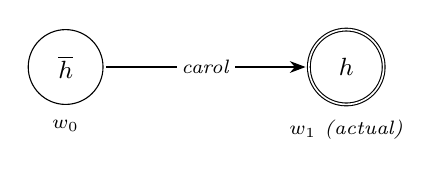
\begin{tikzpicture}[node distance=26mm]
  \node[world] (w0) {$\overline{h}$};
  \node[actual, right=of w0] (w1) {$h$};
  \draw[plaus] (w0) -- node[elab] {\emph{carol}} (w1);
  \node[wlab, below=1.5mm of w0] {$w_0$};
  \node[wlab, below=1.5mm of w1] {$w_1$ (actual)};
\end{tikzpicture}
\caption{The initial Coin Lie model. The double ring marks the actual world. The arrow is
Carol's plausibility relation and points toward the \emph{more} plausible world, so she
believes $h$ without knowing it. Alice and Bob have no arrow between the worlds, which is
what it means for them to know the coin: each of their relations is the identity.}
\label{fig:initial}
\end{figure}

Read off \Cref{fig:initial}: $\Kop{\mathit{alice}} h$ holds, because every world Alice
cannot rule out---just $w_1$---has $h$. $\Kop{\mathit{carol}} h$ fails, because Carol
cannot rule out $w_0$. $\Bop{\mathit{carol}} h$ holds, because $w_1$ is the more plausible
of the two. That one picture already separates knowledge from belief, and
\Cref{sec:logic} makes the separation precise.

\subsection{Contributions}

\begin{enumerate}
  \item \textbf{A formalisation of \mBplus} (\Cref{sec:logic}), extending \mB{}
    \citep{buckingham2021thesis} with safe belief $\Sop{i}$ and conditional belief
    $\CBop{i}{\psi}$, taken from Baltag and Smets \citep{baltag2008}, together with
    conditional ontic effects. We are explicit that the operators are not new; what is new
    is their presence in the object language of an action formalism, where they become
    queryable properties of a planning state.

  \item \textbf{A surface language} (\Cref{sec:surface}) in which initial states are given
    \emph{declaratively}---as a list of facts and attitudes that the model must
    satisfy---rather than as a hand-drawn Kripke structure, together with non-recursive
    definitions, Horn rules over static constants, and state invariants.

  \item \textbf{A query language and enumeration procedure} (\Cref{sec:query}). Queries are
    formulas of the full modal language extended with a hole $\hole$; enumeration ranges over
    modal literals to depth $d$, following the representation of \citet{muise2015}. Repeated
    holes are filled uniformly, which is what allows a single pattern to express ``what does
    $a$ believe that is false'' as $\Bop{a}\hole \wedge \neg\hole$.

  \item \textbf{An implementation and its measurement} (\Cref{sec:impl,sec:eval}). We report
    the effect of bisimulation contraction on iterated update and show that, while it
    converts exponential growth into a fixed point on several standard domains, there are
    domains on which it demonstrably does not.

  \item \textbf{An explicit accounting} (\Cref{sec:related}) of which parts of the system are
    transcribed from the literature and which are new, including three points at which the
    source documents disagree with each other and the resolution adopted.
\end{enumerate}

\subsection{Scope}

\delhi{} is a model checker, not a planner and not a theorem prover. It answers whether a
formula holds in a given finite state, and computes the state resulting from a named action.
It does not search for a sequence of actions achieving a goal; plan existence in the general
dynamic-epistemic setting is undecidable \citep{bolander2011}, and the restrictions that
recover decidability are orthogonal to the semantic questions treated here. Validity across
all models is likewise out of scope: every judgement reported is a judgement about a
particular pointed model.

Two assumptions run through the whole development and are worth stating before they are used
rather than after.

\textbf{The analyst knows which world is actual.} A pointed model designates one world, and
the modeller supplies it. Every judgement involving $\Sop{i}$ depends on that designation,
since safe belief is measured from the actual world outward---so $\Sop{i}$ is available to
someone reasoning \emph{about} the scenario and, as \Cref{thm:introspect} makes precise, not
to an agent reasoning inside it. Where the actual world is itself uncertain, the framework as
presented does not apply.

\textbf{Domains are small enough for explicit-state checking.} Models are represented
extensionally, as sets of worlds with bitset valuations and relations. This is what makes the
measurements of \Cref{sec:eval} meaningful and also what bounds them: the approach suits
scenarios of the size found in the theory-of-mind and epistemic-planning literature---tens to
a few thousand worlds---and not domains requiring symbolic or factored representation.

% ===========================================================================
\section{Preliminaries}
\label{sec:prelim}

We assume finite sets $\Props$ of propositional atoms and $\Ag$ of agents.

\subsection{Plausibility models}

The central object is a Kripke structure in which each agent's accessibility relation is a
\emph{preorder} rather than an equivalence, read as a comparative judgement of plausibility.

\begin{definition}[Plausibility model]
\label{def:model}
A \emph{plausibility model} is a triple $M = \langle \Worlds, R, V\rangle$ where
\begin{itemize}
  \item $\Worlds$ is a finite non-empty set of \emph{worlds};
  \item $R : \Worlds \times \Worlds \to (\Ag \to \mathbb{B})$, written $u \plaus{i} v$ for
    $R(u,v)(i) = \mathrm{true}$ and read \emph{``agent $i$ considers $v$ at least as
    plausible as $u$''};
  \item $V : \Props \to 2^{\Worlds}$ is a valuation.
\end{itemize}
Each $\plaus{i}$ is required to be \emph{locally well-preordered}: a preorder (reflexive and
transitive) whose restriction to any comparability class is connected. A \emph{state} is a
pointed model $\langle M, u\rangle$ with $u \in \Worlds$ the \emph{actual} world.
\end{definition}

\begin{remark}[Direction of the ordering]
\label{rem:direction}
Plausibility \emph{increases} along the arrow: $u \plaus{i} v$ says $v$ is the more credible
of the two. This convention is worth stating explicitly because a model built with the
relation inverted is still a well-formed model---it satisfies every frame condition of
\Cref{def:model}---so no structural validation can detect the error. Every answer the system
gives will simply be reversed.
\end{remark}

Two relations are derived from $\plaus{i}$, and the whole of the semantics rests on the
contrast between them.

\begin{definition}[Comparability and maxima]
\label{def:derived}
For a plausibility model $M$, agent $i$, world $u$ and $C \subseteq \Worlds$:
\begin{align}
  u \comp{i} v \quad&\text{iff}\quad u \plaus{i} v \ \text{ or }\ v \plaus{i} u,
    &&\text{(comparability)}\\
  \comp{i}^{u} \ &\coloneqq\ \{\, v \mid u \comp{i} v \,\},
    &&\text{(the class of $u$)}\\
  \best{i} C \ &\coloneqq\ \{\, u \in C \mid u' \plaus{i} u \text{ for all } u' \in C \,\},
    &&\text{(maxima of $C$)}\\
  \best{i}^{u} \ &\coloneqq\ \best{i} \comp{i}^{u}. &&
\end{align}
\end{definition}

\begin{proposition}
$\comp{i}$ is an equivalence relation on $\Worlds$.
\end{proposition}

\begin{proof}
Reflexivity and symmetry are immediate from the definition and the reflexivity of
$\plaus{i}$. For transitivity, suppose $u \comp{i} v$ and $v \comp{i} w$. Local connectedness
makes $\plaus{i}$ total on the comparability class containing $u$ and $v$, and $v$ and $w$
lie in that same class; hence $u$ and $w$ are comparable.
\end{proof}

\begin{proposition}[Non-emptiness of maxima]
\label{prop:nonempty}
If $C$ is a non-empty finite subset of a single comparability class, then $\best{i} C \neq
\emptyset$.
\end{proposition}

\begin{proof}
Local connectedness makes $\plaus{i}$ restricted to that class a total preorder. A finite
non-empty total preorder has maximal elements.
\end{proof}

\begin{remark}[A precondition that must not be dropped]
\label{rem:nonempty}
Proposition~\ref{prop:nonempty} is stated in \citet{buckingham2021thesis} without the single-class
restriction, and in that generality it is false: if $C$ contains worlds drawn from two
distinct comparability classes, no element of either is $\plaus{i}$-related to any element of
the other, so $\best{i} C = \emptyset$. Both uses of $\best{i}$ in \mBplus{} respect the
restriction---$\best{i}\comp{i}^{u}$ takes a whole class, and the conditional-belief case of
\Cref{def:sat} intersects a class with a denotation and treats the empty case
explicitly---but an implementation that asserts non-emptiness unconditionally will fail on
inputs the semantics permits.
\end{remark}

\subsection{Why one relation and not two}

An alternative design gives each agent two relations, one equivalence for knowledge and one
serial-transitive-Euclidean relation for belief, and constrains them to interact. The
plausibility approach derives both from a single preorder, which has two consequences that
matter for this paper.

First, the interaction axioms come for free rather than being imposed. Because $\best{i}^{u}
\subseteq \comp{i}^{u}$ by construction, $\Kop{i}\varphi \to \Bop{i}\varphi$ is valid on every
model, and no separate frame condition is required to secure it.

Second---and this is the point of the exercise---belief revision becomes a \emph{reordering}
rather than a deletion. Learning that $\psi$ does not remove the $\neg\psi$-worlds from the
model; it promotes the $\psi$-worlds above them. The agent's knowledge is therefore unchanged
by an announcement, while its belief may be overturned, and because the demoted worlds are
still present, a subsequent truthful announcement can promote them back. A semantics that
deleted worlds would make the first lie irreversible.

% ===========================================================================
\section{The logic \mBplus}
\label{sec:logic}

\subsection{Syntax}

\begin{definition}[Formula language]
\label{def:syntax}
The language $\Lgb$ is generated by
\[
  \varphi \ ::=\ p \ \mid\ \neg\varphi \ \mid\ \varphi \wedge \varphi
    \ \mid\ \Kop{i}\varphi \ \mid\ \Bop{i}\varphi \ \mid\ \Cop{g}\varphi
    \ \mid\ \CBop{i}{\psi}\varphi \ \mid\ \Sop{i}\varphi
\]
with $p \in \Props$, $i \in \Ag$, $g \subseteq \Ag$, and $\psi \in \Lgb$. We write $\Lprop$
for the propositional fragment (the first three clauses). The connectives $\vee$,
$\rightarrow$, $\top$ and $\bot$ are defined as usual.
\end{definition}

The first six clauses are those of \mB{} \citep[Def.~1]{buckingham2021thesis}. The last two,
conditional belief and safe belief, are the extension marked by the $+$; they are Baltag and
Smets's operators \citep{baltag2006,baltag2008}, and were already interpretable in \mB's
models, since those models \emph{are} plausibility models. What \mB{} does not do is lift them
into its object language. \mBplus{} does.

\subsection{Semantics}

\begin{definition}[Satisfaction]
\label{def:sat}
For a state $\langle M, u\rangle$ with $M = \langle \Worlds, R, V\rangle$:
\begin{align}
  \langle M,u\rangle &\models p
    &&\text{iff}\quad u \in V(p) \\
  \langle M,u\rangle &\models \neg\varphi
    &&\text{iff}\quad \langle M,u\rangle \not\models \varphi \\
  \langle M,u\rangle &\models \varphi \wedge \chi
    &&\text{iff}\quad \langle M,u\rangle \models \varphi
       \text{ and } \langle M,u\rangle \models \chi \\
  \langle M,u\rangle &\models \Kop{i}\varphi
    &&\text{iff}\quad \langle M,v\rangle \models \varphi
       \text{ for all } v \in \comp{i}^{u} \\
  \langle M,u\rangle &\models \Bop{i}\varphi
    &&\text{iff}\quad \langle M,v\rangle \models \varphi
       \text{ for all } v \in \best{i}^{u} \\
  \langle M,u\rangle &\models \Sop{i}\varphi
    &&\text{iff}\quad \langle M,v\rangle \models \varphi
       \text{ for all } v \text{ with } u \plaus{i} v \\
  \langle M,u\rangle &\models \CBop{i}{\psi}\varphi
    &&\text{iff}\quad \langle M,v\rangle \models \varphi
       \text{ for all } v \in \best{i}\!\left(\comp{i}^{u} \cap \denote{\psi}\right) \\
  \langle M,u\rangle &\models \Cop{g}\varphi
    &&\text{iff}\quad \langle M,v\rangle \models \varphi
       \text{ for all } v \text{ with } u \left(\textstyle\bigcup_{i \in g} \comp{i}\right)^{*} v
\end{align}
where $\denote{\psi} = \{v \mid \langle M,v\rangle \models \psi\}$ and $(\cdot)^{*}$ denotes
reflexive-transitive closure. The conditional-belief clause is vacuously true when
$\comp{i}^{u} \cap \denote{\psi} = \emptyset$.
\end{definition}

Three points deserve comment.

\paragraph{Common knowledge, not common belief.}
$\Cop{g}$ is built on $\comp{i}$, the comparability relation, and is therefore common
\emph{knowledge}. Some presentations use the same symbol for the closure over $\plaus{i}$,
which yields common \emph{belief}; the two are not interchangeable, and \delhi{} implements
the knowledge reading throughout.

\paragraph{$\Bop{i}$ is a special case of $\CBop{i}{\psi}$.}
Taking $\psi = \top$ gives $\comp{i}^{u} \cap \Worlds = \comp{i}^{u}$, so
$\CBop{i}{\top}\varphi \equiv \Bop{i}\varphi$. The implementation tests this identity rather
than assuming it.

\paragraph{Safe belief is anchored to the actual world.}
$\Kop{i}$ quantifies over a fixed set (the class), $\Bop{i}$ over another fixed set (the
maxima). $\Sop{i}$ quantifies over $\{v : u \plaus{i} v\}$, which depends on \emph{where $u$
sits} in the ordering. This gives $\Sop{i}$ a character quite unlike the other two, developed
in \Cref{sec:safe}.

\subsection{The strength hierarchy}

\begin{theorem}[Hierarchy]
\label{thm:hierarchy}
For every model, agent and formula,
\[
  \Kop{i}\varphi \ \rightarrow\ \Sop{i}\varphi \ \rightarrow\ \Bop{i}\varphi ,
\]
and neither implication is reversible.
\end{theorem}

\begin{proof}
The three operators quantify over $\comp{i}^{u} \supseteq \{v : u \plaus{i} v\} \supseteq
\best{i}^{u}$. The first inclusion holds because $u \plaus{i} v$ implies $u \comp{i} v$. The
second holds because a maximal element of the class is $\plaus{i}$-above every element of it,
$u$ included. A larger quantification domain yields a stronger claim, giving both
implications. Failure of the converses is witnessed in Example~\ref{ex:safe}.
\end{proof}

\Cref{fig:nested} is the same statement as a picture, and it is worth keeping in mind for
the rest of the paper: the three attitudes differ only in how much of the agent's
comparability class they are required to survive.

\begin{figure}[t]
\centering
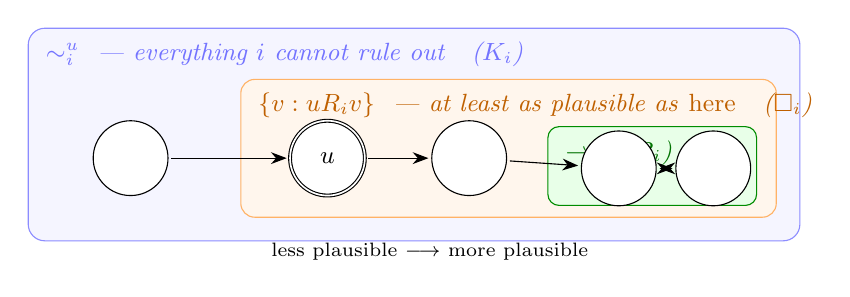
\begin{tikzpicture}[scale=1.0]
  % outermost: the comparability class
  \draw[rounded corners=6pt, fill=blue!4, draw=blue!45]
    (-0.2,-0.2) rectangle (9.6,2.5);
  \node[anchor=north west, font=\small\itshape, blue!55] at (-0.1,2.45)
    {$\comp{i}^{u}$ \ --- everything $i$ cannot rule out \ \ ($\Kop{i}$)};

  % middle: the up-set from u
  \draw[rounded corners=5pt, fill=orange!7, draw=orange!60]
    (2.5,0.1) rectangle (9.3,1.85);
  \node[anchor=north west, font=\small\itshape, orange!75!black] at (2.6,1.8)
    {$\{v : u \plaus{i} v\}$ \ --- at least as plausible as \emph{here} \ \ ($\Sop{i}$)};

  % inner: the maxima
  \draw[rounded corners=4pt, fill=green!9, draw=green!55!black]
    (6.4,0.25) rectangle (9.05,1.25);
  \node[anchor=north west, font=\small\itshape, green!45!black] at (6.5,1.2)
    {$\best{i}^{u}$ \ ($\Bop{i}$)};

  % worlds, least plausible on the left
  \node[world, fill=white] (a) at (1.1,0.85) {};
  \node[actual, fill=white] (b) at (3.6,0.85) {$u$};
  \node[world, fill=white] (c) at (5.4,0.85) {};
  \node[world, fill=white] (d) at (7.3,0.72) {};
  \node[world, fill=white] (e) at (8.5,0.72) {};
  \draw[plaus] (a) -- (b);
  \draw[plaus] (b) -- (c);
  \draw[plaus] (c) -- (d);
  \draw[equi] (d) -- (e);
  \node[font=\scriptsize, anchor=north] at (4.9,-0.1) {less plausible $\longrightarrow$ more plausible};
\end{tikzpicture}
\caption{The three attitudes as three nested quantification domains, drawn for one agent
$i$ at the actual world $u$. $\Kop{i}$ reads the whole class, $\Bop{i}$ only the maxima, and
$\Sop{i}$ the worlds from $u$ upward. Because the middle region is pinned to $u$, it shrinks
as the agent's belief becomes more accurate---which is the asymmetry developed in
\Cref{sec:safe}.}
\label{fig:nested}
\end{figure}

\begin{theorem}[Frame properties]
\label{thm:frames}
On every plausibility model:
\begin{enumerate}
  \item $\Kop{i}$ satisfies $T$, $4$ and $5$, hence is an $S5$ modality;
  \item $\Bop{i}$ satisfies $D$, $4$ and $5$, hence is a $KD45$ modality, and does
    \emph{not} satisfy $T$;
  \item $\Sop{i}$ is factive: $\Sop{i}\varphi \to \varphi$. It satisfies $4$ but \emph{not}
    $5$, and is therefore $S4$ rather than $S5$---see Proposition~\ref{prop:s4};
  \item $\Kop{i}\varphi \to \Bop{i}\varphi$, $\Bop{i}\varphi \to \Kop{i}\Bop{i}\varphi$, and
    $\Kop{i}\varphi \to \Sop{i}\varphi$.
\end{enumerate}
\end{theorem}

\begin{proof}[Proof sketch]
(1) is immediate from $\comp{i}$ being an equivalence relation. (2): seriality follows from
Proposition~\ref{prop:nonempty} applied to $\comp{i}^{u}$, which is non-empty since $u \comp{i} u$;
introspection follows because $\best{i}^{u}$ depends only on the class of $u$, and all worlds
in a class have the same class. Failure of $T$ is witnessed by any model in which $u \notin
\best{i}^{u}$. (3): reflexivity of $\plaus{i}$ places $u$ in its own quantification domain.
(4): the inclusions of Theorem~\ref{thm:hierarchy}, plus the class-invariance of $\best{i}^{u}$ for
the second conjunct.
\end{proof}

\begin{remark}
The asymmetry in (2)---consistency but not factivity---is the formal content of the informal
claim that an agent may be \emph{wrong but not incoherent}. $\Bop{i}\varphi \wedge \neg\varphi$
is satisfiable; $\Bop{i}\varphi \wedge \Bop{i}\neg\varphi$ is not.
\end{remark}

\subsection{Derived attitudes}
\label{sec:sugar}

The implemented core has exactly the eight cases of \Cref{def:sat}. Every further attitude
in \Cref{tab:sugar} is defined by translation and eliminated before evaluation.

\begin{table}[t]
\centering
\begin{tabular}{@{}llll@{}}
\toprule
\textbf{Surface} & \textbf{Notation} & \textbf{Definition} & \textbf{Reading} \\
\midrule
\code{K'[a]}$\varphi$  & $\hat{K}_a\varphi$ & $\neg\Kop{a}\neg\varphi$ & considers possible \\
\code{B'[a]}$\varphi$  & $\hat{B}_a\varphi$ & $\neg\Bop{a}\neg\varphi$ & does not rule out \\
\code{S'[a]}$\varphi$  & $\hat{S}_a\varphi$ & $\neg\Sop{a}\neg\varphi$ & safe-belief dual \\
\code{Kw[a]}$\varphi$  & $\Kw{a}\varphi$    & $\Kop{a}\varphi \vee \Kop{a}\neg\varphi$ & knows whether \\
\code{Bw[a]}$\varphi$  & $\Bw{a}\varphi$    & $\Bop{a}\varphi \vee \Bop{a}\neg\varphi$ & believes whether \\
\code{?[a]}$\varphi$   & $\Ig{a}\varphi$    & $\neg \Kw{a}\varphi$ & ignorant whether \\
\code{??[a]}$\varphi$  & $\Susp{a}\varphi$  & $\neg \Bw{a}\varphi$ & suspends judgement \\
\code{C[*]}$\varphi$   & $\Cop{\Ag}\varphi$ & $\Cop{g}\varphi$, $g = \Ag$ & common knowledge \\
\code{K[a,b]}$\varphi$ & --- & $\Kop{a}\varphi \wedge \Kop{b}\varphi$ & agent-list distribution \\
\bottomrule
\end{tabular}
\caption{Derived attitudes. Agent lists distribute over $K$, $B$, $\Box$, $\mathit{Kw}$,
$\mathit{Bw}$, $?$ and $??$. Each is a Boolean combination of the primitives, so the
evaluator implements eight cases and no more.}
\label{tab:sugar}
\end{table}

The ``whether'' operators are worth singling out. $\Kw{a}\varphi$ is not $\Kop{a}\varphi$ and
not its negation: it is a \emph{disjunction} of two knowledge claims, asserting that the agent
has settled the question without saying which way. Questions about ignorance are its negation.
That these require a disjunction is what makes them operators rather than abbreviations a user
can be expected to expand by hand, and \Cref{sec:query} shows that the same disjunctive
structure is what lets the enumeration procedure reach them.

\subsection{Safe belief}
\label{sec:safe}

Safe belief occupies the gap in Theorem~\ref{thm:hierarchy}, and because it is measured from the
actual world its behaviour is asymmetric in a way worth developing.

\subsubsection{Background: safe belief in Baltag and Smets}
\label{sec:bsbackground}

The operator is not ours and neither is the name. \citet{baltag2006,baltag2008} introduce
\emph{safe belief} on plausibility models as part of a programme separating knowledge, belief
and plausibility and giving each its own dynamics. Three features of their treatment matter
for how we use it, and the third is the one most easily missed.

\textbf{It is offered as a notion of knowledge, not as a strong belief.} Baltag and Smets
present safe belief as a \emph{weak, non-negatively-introspective} kind of knowledge---an
alternative to the $S5$ reading rather than a way-station between $S5$ and $KD45$. The
motivation is the defeasibility tradition of \citet{lehrer1969} and \citet{stalnaker2006}:
knowledge as true belief that no further truth would overturn, which is exactly
Proposition~\ref{prop:defeasible}.

\textbf{Its logic is axiomatised alongside conditional belief.} Their work gives complete
axiomatisations for knowledge, conditional belief and safe belief over plausibility models,
and develops the dynamics---how each attitude moves under action-priority update---together
with quantitative refinements such as degrees of safety.

\textbf{It is $S4$, not $S5$.} This is the technical content of ``non-negatively
introspective'', and it separates safe belief sharply from both of its neighbours.

\begin{proposition}[Safe belief is $S4$]
\label{prop:s4}
$\Sop{i}$ is a normal modality satisfying $T$ and $4$ but not $5$: $\Sop{i}\varphi \to
\varphi$ and $\Sop{i}\varphi \to \Sop{i}\Sop{i}\varphi$ are valid, while
$\neg\Sop{i}\varphi \to \Sop{i}\neg\Sop{i}\varphi$ is not.
\end{proposition}

\begin{proof}
Normality is immediate, $\Sop{i}$ being a box over $\plaus{i}$; $T$ follows from reflexivity
and $4$ from transitivity (both appear in Theorem~\ref{thm:introspect}). For the failure of
$5$, take $\Worlds = \{w_0, w_1\}$ with $\denote{p} = \{w_1\}$, $w_0 \plaus{i} w_1$, and
$w_0$ actual---an agent whose most plausible world satisfies $p$ while the actual world does
not. At $w_0$ the up-set is $\{w_0,w_1\}$ and $p$ fails at $w_0$, so $\neg\Sop{i}p$ holds.
But $w_1$ is maximal, so its up-set is $\{w_1\}$, where $p$ holds; hence $\Sop{i}p$ holds at
$w_1$, $\neg\Sop{i}p$ fails there, and $\Sop{i}\neg\Sop{i}p$ fails at $w_0$.
\end{proof}

\begin{remark}[Where the three attitudes part company]
\label{rem:axioms}
In the model of Proposition~\ref{prop:s4}, $\Kop{i}$ and $\Bop{i}$ both satisfy $5$ and
$\Sop{i}$ does not, so the failure is a property of safe belief and not of the model. This is
the precise sense in which safe belief is a \emph{weaker} knowledge: it keeps factivity,
which belief lacks, and gives up negative introspection, which knowledge has. An agent with
$\Sop{i}$ need not be aware of the boundaries of its own safe beliefs---and
\Cref{sec:introspect} establishes the stronger fact that it cannot determine them at all.
\end{remark}

\paragraph{What \mBplus{} adds.}
The operator, its characterisation and its axiomatisation are Baltag and Smets's. What we
contribute is its \emph{availability inside an action formalism}. In \mB{} and its relatives
the plausibility models already interpret $\Sop{i}$ and $\CBop{i}{\psi}$, but the object
language of the action description does not mention them, so they cannot appear in a goal, an
invariant, or a query. Lifting them makes safe belief a property one can \emph{check of a
planning state}, which in turn makes two questions askable that were not before: which actions
confer it (\Cref{sec:acquisition}), and whether an agent can establish it of itself
(\Cref{sec:introspect}). The answer to the second is the negative result of
Theorem~\ref{thm:introspect}, and it is not in the source literature.

\begin{example}[Three positions on one question]
\label{ex:safe}
Consider $\Props = \{\mathit{up}\}$ and three agents, none of whom knows the answer:
\begin{lstlisting}
initially {
    up                        // the server really is up
    ?[ada] up   B[ada] up     // ada cannot tell, but leans the right way
    ?[ben] up   B[ben] !up    // ben cannot tell, and leans the wrong way
    ?[cleo] up                // cleo has no leaning either way
}
\end{lstlisting}
Then $\Bop{\mathit{ada}}\,\mathit{up}$ and $\Bop{\mathit{ben}}\,\neg\mathit{up}$ both hold, so
belief cannot separate the first two agents. Safe belief separates all three:
$\Sop{\mathit{ada}}\,\mathit{up}$ holds, $\Sop{\mathit{ben}}\,\neg\mathit{up}$ does not
(indeed cannot, by factivity), and $\Sop{\mathit{cleo}}\,\mathit{up}$ does not, because both
worlds are maximal for \emph{cleo} and so both lie above the actual one.
\end{example}

\begin{proposition}[Defeasibility characterisation]
\label{prop:defeasible}
$\Sop{i}\varphi$ holds at $\langle M,u\rangle$ if and only if $\CBop{i}{\psi}\varphi$ holds
at $\langle M,u\rangle$ for every $\psi$ with $\langle M,u\rangle \models \psi$.
\end{proposition}

\begin{proof}
$(\Rightarrow)$ Assume $\Sop{i}\varphi$ at $u$, so $\varphi$ holds throughout $U \coloneqq
\{v : u \plaus{i} v\}$. Let $\psi$ be true at $u$ and let $v \in
\best{i}(\comp{i}^{u} \cap \denote{\psi})$. Since $u \in \comp{i}^{u} \cap \denote{\psi}$,
that set is non-empty, and by maximality of $v$ within it we have $u \plaus{i} v$. Hence $v
\in U$ and $\varphi$ holds at $v$. As $v$ was arbitrary, $\CBop{i}{\psi}\varphi$ holds.

$(\Leftarrow)$ Contrapositive. Suppose $\Sop{i}\varphi$ fails, so there is $w$ with $u
\plaus{i} w$ and $\varphi$ false at $w$. Take $\psi$ to be true exactly at $w$ and at the
worlds of $\comp{i}^{u}$ ranked no higher than $w$ --- concretely, $\denote{\psi} \cap
\comp{i}^{u} = \{v \in \comp{i}^{u} : v \plaus{i} w\}$, which is expressible whenever the
model is finite and worlds are distinguished by atoms, and which contains $u$ because $u
\plaus{i} w$. Then $\psi$ is true at $u$, and $w$ is $\plaus{i}$-maximal in $\comp{i}^{u}
\cap \denote{\psi}$ by construction, so $w \in \best{i}(\comp{i}^{u} \cap \denote{\psi})$.
Since $\varphi$ fails at $w$, $\CBop{i}{\psi}\varphi$ fails.
\end{proof}

\begin{remark}[Reading the characterisation]
This is the property that makes $\Sop{i}$ more than a technical interpolant: \emph{a safe
belief is one that no true information can overturn}, since conditioning on a true $\psi$ is
exactly what a truthful announcement of $\psi$ does to the ordering. The restriction to
\emph{true} $\psi$ is not decoration --- a safe belief may still be overturned by a
falsehood, and \Cref{sec:acquisition} exhibits a case. The $(\Leftarrow)$ direction requires
that the separating $\psi$ be expressible, which holds in the finite, atom-distinguished
models \delhi{} constructs; over models where worlds are not separated by any formula the
implication may fail, and $\Sop{i}$ is then strictly stronger than the conditional-belief
conjunction.
\end{remark}

\subsubsection{Introspection}
\label{sec:introspect}

Because $\Sop{i}$ is anchored to the actual world, and the actual world is precisely what an
agent cannot locate, safe belief is not introspectible in the way knowledge and belief are.

\begin{theorem}[Introspection collapse]
\label{thm:introspect}
On every plausibility model:
\[
  \Kop{i}\Sop{i}\varphi \ \equiv\ \Kop{i}\varphi,
  \qquad
  \Bop{i}\Sop{i}\varphi \ \equiv\ \Bop{i}\varphi,
  \qquad
  \Sop{i}\Sop{i}\varphi \ \equiv\ \Sop{i}\varphi .
\]
\end{theorem}

\begin{proof}
\emph{First.} $(\Leftarrow)$ If $\varphi$ holds throughout $\comp{i}^{u}$ then in particular it
holds throughout every up-set contained in that class, so $\Sop{i}\varphi$ holds at every $v
\in \comp{i}^{u}$. $(\Rightarrow)$ Suppose $\Kop{i}\Sop{i}\varphi$ at $u$, and let $v_0$ be a
minimal element of $\comp{i}^{u}$, which exists because the class is finite and, by local
connectedness, totally preordered. Then $\{w : v_0 \plaus{i} w\} = \comp{i}^{u}$, and
$\Sop{i}\varphi$ at $v_0$ gives $\varphi$ throughout the class, i.e.\ $\Kop{i}\varphi$ at $u$.

\emph{Second.} Let $v \in \best{i}^{u}$. Since $v$ is maximal in its class, $\{w : v \plaus{i}
w\} = \best{i}^{u}$. Hence $\Sop{i}\varphi$ at $v$ iff $\varphi$ holds throughout
$\best{i}^{u}$, which is $\Bop{i}\varphi$ at $u$; and this is independent of the choice of $v$.

\emph{Third.} Transitivity of $\plaus{i}$ gives $\Sop{i}\varphi \to \Sop{i}\Sop{i}\varphi$;
reflexivity gives the converse.
\end{proof}

\begin{corollary}[Overconfidence]
\label{cor:overconfident}
Every agent believes each of its beliefs to be safe: $\Bop{i}\varphi \to
\Bop{i}\Sop{i}\varphi$ is valid, including when $\Sop{i}\varphi$ is false.
\end{corollary}

\begin{proof}
Immediate from the second equivalence of Theorem~\ref{thm:introspect}, which gives
$\Bop{i}\Sop{i}\varphi \equiv \Bop{i}\varphi$ and hence the implication in both directions.
That the consequent may hold while $\Sop{i}\varphi$ is false is witnessed in
Example~\ref{ex:safe}: $\Bop{\mathit{ben}}\Sop{\mathit{ben}}\neg\mathit{up}$ holds because
$\Bop{\mathit{ben}}\neg\mathit{up}$ does, while $\Sop{\mathit{ben}}\neg\mathit{up}$ fails by
factivity, $\neg\mathit{up}$ being false at the actual world.
\end{proof}

Corollary~\ref{cor:overconfident} is not a defect of the semantics but a consequence of belief being
evaluated at the maxima: from the top of one's own ordering, every belief looks unshakeable.
In Example~\ref{ex:safe}, $\Bop{\mathit{ben}}\Sop{\mathit{ben}}\neg\mathit{up}$ holds while
$\Sop{\mathit{ben}}\neg\mathit{up}$ does not; \emph{ben} takes his belief to be immune to
revision at the moment before one true announcement overturns it.

The practical consequence for modelling is that $\Sop{i}$ is an \emph{external} operator. It
measures the fit between an agent's ordering and the actual world; the agent has no access to
the second argument, and its self-report is uninformative because it is unconditionally
affirmative. An analyst may ask $\Sop{i}\varphi$ of a state; an agent may not ask it of itself.

\begin{remark}[Why the operator is worth having at all]
\label{rem:defeasibility}
$\Kop{i}$ here is $S5$: infallible certainty, true in every world the agent cannot rule out.
A long tradition in epistemology holds that this is too strong for the ordinary word
\emph{knows}, and proposes instead that knowledge is true belief that no further truth would
overturn---the \emph{defeasibility analysis} of \citet{lehrer1969}, developed by
\citet{stalnaker2006}. By Proposition~\ref{prop:defeasible} that analysis is exactly
$\Sop{i}$. Safe belief is therefore not a technical interpolant wedged between two real
operators; it is a serious candidate for what knowing \emph{is}, and \mBplus{} carries both
readings in one model so that a modeller may ask for either and compare them.
\end{remark}

\subsubsection{How safe belief is acquired}
\label{sec:acquisition}

An agent safely believes $\varphi$ exactly when the actual world is ranked at least as high as
every world where $\varphi$ fails. \Cref{tab:acquire} records the three dynamic routes,
anticipating the action layer of \Cref{sec:dynamics}.

\begin{table}[t]
\centering
\begin{tabular}{@{}llccc@{}}
\toprule
\textbf{Route} & \textbf{Instance} & $\Kop{i}$ & $\Sop{i}$ & $\Bop{i}$ \\
\midrule
Sensing              & the agent looks                   & \checkmark & \checkmark & \checkmark \\
Truthful announcement & the agent is told, and it is true & ---        & \checkmark & \checkmark \\
Lie                   & the agent is told a falsehood     & ---        & ---        & \checkmark \\
\bottomrule
\end{tabular}
\caption{Acquisition of the three attitudes toward the announced proposition. The middle row
is the case that motivates the operator: a truthful announcement upgrades a previously
mistaken belief to a safe one without conferring knowledge.}
\label{tab:acquire}
\end{table}

Two observations. First, the middle row describes a state with no compact name in ordinary
usage: the agent is now right, no true information can dislodge it, and it still cannot rule
out the alternative. Second, the bottom row cannot come out otherwise, since $\Sop{i}$ is
factive---but a lie can nevertheless \emph{destroy} a safe belief, by reordering the worlds of
an agent that previously held one. Safety is immunity to truth, not permanence.

% ===========================================================================
\section{The surface language}
\label{sec:surface}

A \delhi{} domain is a text file with a fixed section structure. We give the grammar, then
treat the sections whose design is not immediate.

\subsection{Structure}

\begin{lstlisting}[caption={Overall file structure. \code{initially} or \code{state} is
required, as is \code{actions}, which may be empty.},captionpos=b]
types      { Actor - Object }        // type hierarchy
objects    { alice, bob - Actor }    // typed constants
agents     { alice, bob }            // which objects have minds
props      { h, d }                  // propositional atoms
constants  { adjacent(hall, study) } // static, world-independent
define     { ... }                   // named formulas, expanded away
rules      { ... }                   // Horn clauses over constants
initially  { ... }                   // declarative initial state
state      { ... }                   //   ...or an explicit model
goal       { phi }                   // optional
invariants { phi ... }               // must hold in every state
actions    { ... }                   // action theory
\end{lstlisting}

\subsection{Declarative initial states}
\label{sec:initially}

The design decision most visible to a user is that initial states are given as
\emph{constraints} rather than as structures. An \code{initially} block lists facts and
attitudes; \delhi{} constructs a model satisfying them and then verifies the model against
every line written.

\begin{lstlisting}
initially {
    h                    // a fact about the actual world
    ?[carol] h           // carol cannot tell whether h
    B[carol] h           // but she correctly leans that way
}
\end{lstlisting}

Anything not mentioned is known by every agent, so the block above yields a two-world model in
which \emph{carol} is uncertain and the others are not. The alternative form, \code{state},
writes the model out directly and is what the tool prints when asked to display one:

\begin{lstlisting}
state {
  *w1 <- { h }          // `*` marks the designated world
   w0 <- { }
  carol: w0 < w1        // w1 is the more plausible
}
\end{lstlisting}

Here \code{<} and \code{<=} point toward the more plausible world and \code{~} relates two
worlds in both directions. Agents with no line distinguish every world, which is to say they
know everything---the degenerate case of \Cref{def:model} in which $\plaus{i}$ is the identity.

\subsection{Definitions, rules and invariants}

Three optional sections address needs that arise in practice and that the underlying
semantics does not itself provide.

\paragraph{Definitions.}
Named formulas, parameterised over objects, expanded before lowering so that the semantics
never encounters the name:
\begin{lstlisting}
define {
    blocked(?r)       = !lit(?r) | locked(?r)
    can_enter(?w, ?r) = !blocked(?r) & K[?w] !blocked(?r)
}
\end{lstlisting}
Parameters may occupy agent positions, as \code{?w} does above. Cycles are rejected when the
definition table is built rather than caught by a depth limit at expansion time. Two
restrictions are deliberate: a defined name may not appear as the target of \code{causes} or
as a world fact, since both require an atom the semantics can \emph{set}; and parameters range
over objects, not formulas, so second-order macros such as \code{define f(?p) = K[a] ?p} are
not admitted.

\paragraph{Rules.}
Horn clauses over the static constant table, saturated to a least fixpoint at parse time:
\begin{lstlisting}
constants { !adjacent(Room, Room)  adjacent(hall, study)  adjacent(study, attic) }
rules {
    reach(?x, ?y) :- adjacent(?x, ?y)
    reach(?x, ?z) :- adjacent(?x, ?y), reach(?y, ?z)
}
\end{lstlisting}
Derived predicates never become propositions, and therefore consume no bit in any world;
\code{reach(hall, attic)} folds to $\top$ exactly as a declared constant would, and ground
actions whose guards fold to $\bot$ are discarded before construction.

The restriction to \emph{constants} is the substantive one. The fixpoint is computed once,
which is sound only because the extension is world-independent. A rule over a fluent would
have an extension varying per world and per action, so evaluating it would require either a
fixpoint per world at query time or the maintenance of derived atoms through product
update---the frame problem in a new place. \delhi{} rejects such rules with a diagnostic
rather than supporting them partially. Bodies carry no negation, keeping the program monotone
so that the least fixpoint exists, and every head variable must occur in the body, so that no
head asserts more than the body justifies.

\paragraph{Invariants.}
Constraints required to hold in \emph{every} state rather than only the first:
\begin{lstlisting}
invariants { !((B[a] p & B[b] !p) | (B[a] !p & B[b] p)) }
\end{lstlisting}
An \code{initially} entry that drives no construction is already an assertion about the start;
an invariant is the same assertion made about the whole run, which is usually what a domain
constraint is intended to mean. Invariants are checked when the initial state is built and
after every action.

% ===========================================================================
\section{Dynamics}
\label{sec:dynamics}

An action changes a state by product update with an event model. The distinguishing feature of
the action-language approach, inherited from \mB{} and $m\mathcal{A}^*$, is that the modeller
does not construct event models: they declare \emph{what changes} and \emph{who observes},
and the event model is derived.

\subsection{Action theories}

\begin{definition}[Action theory]
\label{def:theory}
An action theory $T$ for action $a$ is a set of statements of the following forms, with the
indicated formula typing:
\begin{center}
\begin{tabular}{@{}clll@{}}
\toprule
\# & \textbf{Form} & \textbf{Typing} & \textbf{Role} \\
\midrule
1 & $a$ \textbf{requires} $\varphi$ & $\varphi \in \Lprop$ & precondition \\
2 & $a$ \textbf{causes} $l_0,\dots,l_n$ \textbf{if} $\varphi$ & $l_j$ literals, $\varphi \in \Lprop$ & ontic effect \\
3 & $a$ \textbf{determines} $\varphi$ & $\varphi \in \Lprop$ & sensing \\
4 & $a$ \textbf{announces} $\psi$ & $\psi \in \Lgb$ & announcement \\
5 & $i$ \textbf{observes} $a$ \textbf{if} $\varphi$ & $\varphi \in \Lprop$ & full observer \\
6 & $i$ \textbf{aware\_of} $a$ \textbf{if} $\varphi$ & $\varphi \in \Lprop$ & partial observer \\
\bottomrule
\end{tabular}
\end{center}
An action theory is \emph{well-formed} when it contains exactly one statement of form 2, 3 or
4; at most one of form 1; no \code{causes} list containing both $p$ and $\neg p$; and, for
every state, no agent satisfying both an \code{observes} and an \code{aware\_of} condition.
\end{definition}

\begin{remark}[Typing is load-bearing]
Form 4 admits a \emph{modal} $\psi$, which need not be true. This is what makes announcements
capable of being lies, and of being about beliefs rather than facts. It also propagates:
announcement event preconditions are $a_{\pre} \wedge \psi$ and are therefore modal, so
precondition evaluation requires full modal entailment against the pre-update model. Edge
conditions, by contrast, remain propositional, being Boolean combinations of observability
conditions---a distinction worth preserving in an implementation, since edge conditions are
evaluated at two worlds per edge per agent and dominate the cost of update.
\end{remark}

\begin{remark}[Preconditions: a divergence in the sources]
\label{rem:pre}
The source documents give three incompatible readings of multiple form-1 statements:
disjunction \citep[eq.~5.1]{buckingham2021thesis}, at most one statement, and---in the
reference implementation's corpus---conjunction. Under the disjunctive reading, \emph{adding}
a precondition makes an action \emph{more} applicable, contradicting both the ordinary meaning
of the word and every domain file in that corpus. \delhi{} adopts the at-most-one rule: a
single \code{pre} clause per action, conjunction written explicitly, and $a_{\pre} = \top$ in
its absence. A second \code{pre} clause is a diagnostic rather than a silent combination.
\end{remark}

\subsection{Observability}
\label{sec:observability}

Each agent occupies exactly one of three positions with respect to an action. The three are
distinguished by two edge labels, defined from the observability conditions of forms 5 and 6:
\begin{align}
  \FPN(i) &\coloneqq \top \\
  \PN(i)  &\coloneqq \neg \textstyle\bigvee_{\text{\code{observes} } \varphi} \varphi \\
  \Nlab(i) &\coloneqq \neg\left(
      \textstyle\bigvee_{\text{\code{observes} } \varphi} \varphi
      \ \vee\
      \textstyle\bigvee_{\text{\code{aware\_of} } \varphi} \varphi \right)
\end{align}

\begin{table}[t]
\centering
\begin{tabular}{@{}llll@{}}
\toprule
\textbf{Position} & \textbf{Declaration} & \textbf{Learns} & \textbf{Labels} \\
\midrule
Full observer   & \code{i observes a}  & what happened, outcome included & $\PN(i)=\bot$, $\Nlab(i)=\bot$ \\
Partial observer& \code{i aware a}     & that it happened, not how       & $\PN(i)=\top$, $\Nlab(i)=\bot$ \\
Oblivious       & neither              & nothing                          & $\PN(i)=\top$, $\Nlab(i)=\top$ \\
\bottomrule
\end{tabular}
\caption{The three observer positions, with the edge labels each induces (for unconditional
declarations). $\PN$ governs whether the agent can distinguish the outcome events; $\Nlab$
governs whether it can distinguish them from the null event.}
\label{tab:observers}
\end{table}

\Cref{tab:observers} makes precise what is otherwise easy to state loosely. A partial observer
retains the edge between the two outcome events---so the outcomes remain indistinguishable to
it---and loses the edge to the null event, so it does rule out that nothing happened. That
combination is exactly the informal reading ``knows the action occurred, not how it turned
out''. The consequence is second-order: if $j$ senses $\varphi$ and $i$ is a partial observer,
$i$ comes to know that $j$ knows \emph{whether} $\varphi$, without learning $\varphi$.

Both declarations admit a condition, evaluated in the state at the time of the action. This is
what \citet{buckingham2021thesis} calls \emph{local dynamic observability}, and it is the
mechanism by which an agent's observer position may change during a trace---for instance, an
agent that is a partial observer only while not distracted.

\subsection{Event models and the three constructions}

\begin{definition}[Action plausibility model]
An \emph{action plausibility model} is $\langle E, Q, \pre, \add, \del, \Gamma\rangle$ with $E$
a finite set of events, $Q : E \times E \to (\Ag \to \Lprop)$ the edge conditions,
$\pre : E \to \Lgb$, $\add, \del : E \to 2^{\Props}$, and $\Gamma \subseteq E$ designated.
Every event carries a reflexive $\FPN$ edge for every agent; unlisted edges are $\bot$.
\end{definition}

\begin{table}[t]
\centering
\small
\begin{tabular}{@{}lp{0.72\textwidth}@{}}
\toprule
\textbf{Kind} & \textbf{Construction} \\
\midrule
Ontic &
$E = \{e^{c}, e^{\top}\}$; $Q(e^{c},e^{\top}) = \Nlab$; $\pre(e^{c}) = a_{\pre}$,
$\pre(e^{\top}) = \top$; $\add(e^{c}) = P^{+}$, $\del(e^{c}) = P^{-}$; $\Gamma = \{e^{c}\}$.
With conditional effects, $e^{c}$ splits into one event per realisable outcome with mutually
exclusive preconditions. \\[0.4em]
Announcement &
$E = \{e^{\varphi}, e^{\neg\varphi}, e^{\top}\}$;
$Q(e^{\varphi},e^{\neg\varphi}) = \PN$, $Q(e^{\neg\varphi},e^{\varphi}) = \FPN$,
$Q(e^{\varphi},e^{\top}) = Q(e^{\neg\varphi},e^{\top}) = \Nlab$;
$\pre(e^{\varphi}) = a_{\pre} \wedge \varphi$, $\pre(e^{\neg\varphi}) = a_{\pre} \wedge
\neg\varphi$, $\pre(e^{\top}) = \top$; $\add = \del = \emptyset$;
$\Gamma = \{e^{\varphi}, e^{\neg\varphi}\}$. \\[0.4em]
Sensing &
As announcement, but $Q(e^{\neg\varphi},e^{\varphi}) = \PN$ rather than $\FPN$. \\
\bottomrule
\end{tabular}
\caption{The three event-model constructions. $P^{+}$ and $P^{-}$ are the positive and
negative literals of the \code{causes} list.}
\label{tab:constructions}
\end{table}

The single-cell difference between announcement and sensing in \Cref{tab:constructions}
carries the whole distinction between being told and finding out, and \Cref{fig:events}
draws it. With $\FPN = \top$ on the backward edge, even a full observer of an announcement
retains an edge from $e^{\neg\varphi}$ to $e^{\varphi}$, and so cannot rule out that what was
said was false; the result is belief. With $\PN$ there, a full observer distinguishes the two
events and comes to \emph{know} whether $\varphi$.

\begin{figure}[t]
\centering
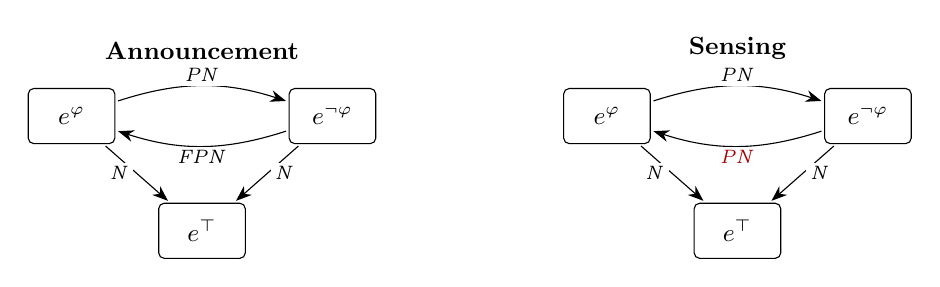
\begin{tikzpicture}[node distance=17mm]
  \begin{scope}
    \node[event] (ap) {$e^{\varphi}$};
    \node[event, right=22mm of ap] (an) {$e^{\neg\varphi}$};
    \node[event, below=11mm of $(ap)!0.5!(an)$] (at) {$e^{\top}$};
    \draw[plaus] (ap) to[bend left=18] node[elab, above] {$\PN$} (an);
    \draw[plaus] (an) to[bend left=18] node[elab, below] {$\FPN$} (ap);
    \draw[plaus] (ap) -- node[elab, left=1pt] {$\Nlab$} (at);
    \draw[plaus] (an) -- node[elab, right=1pt] {$\Nlab$} (at);
    \node[font=\small\bfseries, above=6mm of $(ap)!0.5!(an)$] {Announcement};
  \end{scope}
  \begin{scope}[xshift=68mm]
    \node[event] (sp) {$e^{\varphi}$};
    \node[event, right=22mm of sp] (sn) {$e^{\neg\varphi}$};
    \node[event, below=11mm of $(sp)!0.5!(sn)$] (st) {$e^{\top}$};
    \draw[plaus] (sp) to[bend left=18] node[elab, above] {$\PN$} (sn);
    % Coloured, not \mathbf: \PN expands to \mathit{PN}, and \mathbf{\mathit{PN}} has no
    % glyph in the maths font -- it renders as a black box.
    \draw[plaus] (sn) to[bend left=18]
      node[elab, below, text=red!65!black] {$\PN$} (sp);
    \draw[plaus] (sp) -- node[elab, left=1pt] {$\Nlab$} (st);
    \draw[plaus] (sn) -- node[elab, right=1pt] {$\Nlab$} (st);
    \node[font=\small\bfseries, above=6mm of $(sp)!0.5!(sn)$] {Sensing};
  \end{scope}
\end{tikzpicture}
\caption{The announcement and sensing event models differ in one edge label, shown in red.
For a full observer $\PN = \bot$ and $\Nlab = \bot$, so under sensing that observer keeps no
edge at all between $e^{\varphi}$ and $e^{\neg\varphi}$ and comes to know which occurred;
under announcement the $\FPN = \top$ edge survives, leaving the possibility that the speaker
lied. Reflexive $\FPN$ edges are present at every event and omitted from the drawing.}
\label{fig:events}
\end{figure}

\subsection{Product update}

\begin{definition}[State transition]
\label{def:update}
Write $e \longrightarrow^{iuv} f$ for $\langle M,u\rangle \models Q(e,f)(i)$ \emph{and}
$\langle M,v\rangle \models Q(e,f)(i)$. The updated model $M' = \langle \Worlds', R',
V'\rangle$ is
\begin{align}
  \Worlds' &= \{\langle u,e\rangle \mid u \in \Worlds,\ e \in E,\
    \langle M,u\rangle \models \pre(e)\} \\
  R'(\langle u,e\rangle,\langle v,f\rangle)(i) &=
    \begin{cases}
      \big(e \longrightarrow^{iuv} f\big) \wedge \neg\big(f \longrightarrow^{iuv} e\big)
        \wedge\ u \comp{i} v, & \text{or} \\
      \big(e \longrightarrow^{iuv} f\big) \wedge \big(f \longrightarrow^{iuv} e\big)
        \wedge\ u \plaus{i} v &
    \end{cases}\\
  V'(\langle u,e\rangle) &= \big(V(u) \cup \add(e)\big) \setminus \del(e)
\end{align}
with designated world $\langle d, e\rangle$ for the unique $e \in \Gamma$ whose precondition
holds at $d$.
\end{definition}

This is Baltag--Smets action-priority update: event plausibility overrides state plausibility,
so incoming information takes precedence over prior belief except where it contradicts prior
knowledge.

\subsubsection{The update worked through}
\label{sec:worked}

\Cref{fig:update} applies \Cref{def:update} to the running example: the initial model of
\Cref{fig:initial} crossed with the announcement model of \Cref{fig:events} for $\psi =
\neg h$.

\begin{figure}[t]
\centering
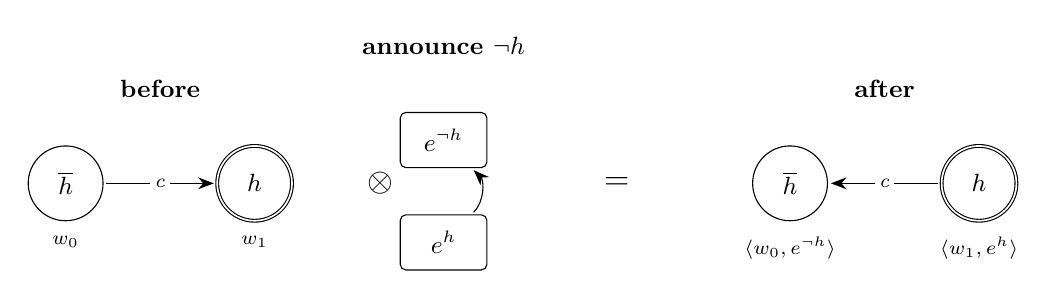
\begin{tikzpicture}
  % ---- before
  \begin{scope}
    \node[world] (w0) at (0,0) {$\overline{h}$};
    \node[actual] (w1) at (2.4,0) {$h$};
    \draw[plaus] (w0) -- node[elab] {\emph{c}} (w1);
    \node[wlab, below=1.5mm of w0] {$w_0$};
    \node[wlab, below=1.5mm of w1] {$w_1$};
    \node[font=\small\bfseries] at (1.2,1.2) {before};
  \end{scope}
  % ---- arrow
  \node at (4.0,0) {\large $\otimes$};
  % ---- event model (announcement of not-h)
  \begin{scope}[xshift=48mm]
    \node[event] (ep) at (0,0.55) {$e^{\neg h}$};
    \node[event] (en) at (0,-0.75) {$e^{h}$};
    % No edge label here: Figure 3 gives the labels, and at this size any label on the
    % arrow collides with it. The caption carries the one fact needed.
    \draw[plaus] (en) to[bend right=45] (ep);
    \node[font=\small\bfseries] at (0,1.75) {announce $\neg h$};
  \end{scope}
  \node at (7.0,0) {\large $=$};
  % ---- after
  \begin{scope}[xshift=92mm]
    \node[world] (p0) at (0,0) {$\overline{h}$};
    \node[actual] (p1) at (2.4,0) {$h$};
    \draw[plaus] (p1) -- node[elab] {\emph{c}} (p0);
    \node[wlab, below=1.5mm of p0] {$\langle w_0, e^{\neg h}\rangle$};
    \node[wlab, below=1.5mm of p1] {$\langle w_1, e^{h}\rangle$};
    \node[font=\small\bfseries] at (1.2,1.2) {after};
  \end{scope}
\end{tikzpicture}
\caption{Alice's lie, worked through. Only the two designated events survive at each world,
since $\pre(e^{\neg h}) = \neg h$ holds only at $w_0$ and $\pre(e^{h}) = h$ only at $w_1$. The
event arrow is the $\FPN$ edge of \Cref{fig:events}, which for Carol makes $e^{\neg h}$
strictly the more plausible event. Carol's world arrow has consequently \emph{reversed}: she
now finds the $\neg h$ world the more plausible, so $\Bop{\mathit{carol}}\neg h$ holds. Her
\emph{knowledge} is untouched---both worlds are still present and still comparable---which is
why \code{peek\_c()} can later restore the truth.}
\label{fig:update}
\end{figure}

The reversal in \Cref{fig:update} is action priority doing its work. The event order says
$e^{\neg h}$ is at least as plausible as $e^{h}$ and not conversely, so the first disjunct of
\Cref{def:update} fires and the event order \emph{overrides} the prior world order.

\begin{proposition}[The two update rules diverge, and the divergence is reachable]
\label{prop:divergence}
Let $\mathrm{R}_{\mathrm{alt}}$ be the rule
\[
  \mathrm{R}_{\mathrm{alt}}(\langle u,e\rangle,\langle v,f\rangle)(i) \ =\
  \big(u \plaus{i} v \wedge (e \to^{iuv} f \vee f \to^{iuv} e)\big) \ \vee\
  \big(v \plaus{i} u \wedge e \to^{iuv} f \wedge \neg (f \to^{iuv} e)\big).
\]
Then $\mathrm{R}_{\mathrm{alt}}$ and \Cref{def:update} agree on three of the four
event-comparability configurations and differ exactly when $f \to^{iuv} e$ holds and $e
\to^{iuv} f$ does not. That configuration is realised in the Coin Lie announcement, and the
two rules give contradictory answers to the goal of \Cref{lst:coinlie}.
\end{proposition}

\begin{proof}
Case analysis on the two edge predicates:
\begin{center}
\begin{tabular}{@{}llll@{}}
\toprule
Configuration & \Cref{def:update} & $\mathrm{R}_{\mathrm{alt}}$ & Agree? \\
\midrule
$e \to f$ and $f \to e$ & $u \plaus{i} v$ & $u \plaus{i} v$ & yes \\
$e \to f$, not $f \to e$ & $u \comp{i} v$ & $u \plaus{i} v \vee v \plaus{i} u = u \comp{i} v$ & yes \\
neither & $\bot$ & $\bot$ & yes \\
\textbf{$f \to e$, not $e \to f$} & $\bot$ & $u \plaus{i} v$ & \textbf{no} \\
\bottomrule
\end{tabular}
\end{center}
For reachability, take $i = \mathit{carol}$, $u = w_1$, $v = w_0$, $e = e^{\neg h}$, $f =
e^{h}$ in \Cref{fig:update}. Carol is a full observer, so $\PN(\mathit{carol}) = \neg\top =
\bot$ and $Q(e^{\neg h}, e^{h})(\mathit{carol}) = \bot$, giving $\neg(e \to f)$; while
$Q(e^{h}, e^{\neg h})(\mathit{carol}) = \FPN = \top$, giving $f \to e$. Also $w_1 \comp{i}
w_0$ and $w_1 \plaus{i} w_0$ fails while $w_0 \plaus{i} w_1$ holds. Under \Cref{def:update}
no edge is created and Carol retains a strict preference for the announced world, so
$\Bop{\mathit{carol}}\neg h$ holds. Under $\mathrm{R}_{\mathrm{alt}}$ the first disjunct
fires, an edge appears in both directions, the worlds become equiplausible, and
$\Bop{\mathit{carol}}\neg h$ fails.
\end{proof}

\begin{remark}[Why this settles the choice]
\label{rem:divergence}
The divergence is not a corner case requiring construction: it is exercised by the very
scenario the source literature uses to \emph{demonstrate} second-order false belief. Under
$\mathrm{R}_{\mathrm{alt}}$ the lie does not land, so the goal of \Cref{lst:coinlie} is
unreachable and the example loses its point. \delhi{} implements \Cref{def:update}; both
rules are implemented behind a feature flag and the configuration above is pinned by a
regression test.
\end{remark}

% ===========================================================================
\section{The query language}
\label{sec:query}

\subsection{Checking}

A query is a formula of $\Lgb$ extended with a hole. Checking is satisfaction:
\[
  \mathrm{eval}(s, \varphi) \ =\ s \models \varphi, \qquad \varphi \in \Lgb ,
\]
total and decidable, since $\models$ is evaluated over a finite model with memoisation.

\begin{lstlisting}[caption={Query grammar. Precedence, loosest to tightest:
\code{->} (right-associative), \code{|}, \code{\&}, \code{!}, modality.},captionpos=b]
query    ::= formula
formula  ::= atom | 'true' | 'false' | '_'
           | '!' formula
           | formula ('&' | '|' | '->') formula
           | modality '[' agents ']' formula
           | 'B' '^' formula '[' agents ']' formula
           | '(' formula ')'
modality ::= 'K' | 'B' | '[]' | 'C' | "K'" | "B'" | "S'"
           | 'Kw' | 'Bw' | '?' | '??'
agents   ::= '*' | name (',' name)*
\end{lstlisting}

The query language is \emph{exactly} the formula language plus $\hole$: every operator of
\Cref{def:sat} and every derived attitude of \Cref{tab:sugar} is available, closed under the
Boolean connectives at arbitrary depth. Goals, invariants and interactive queries share one
parser and one lowering path, so nothing expressible as a goal is inexpressible as a query.

\begin{remark}[The hole is a token]
$\hole$ lexes as a distinct token; \code{\_x} and \code{at\_park} remain ordinary identifiers.
This is load-bearing rather than cosmetic. Filling by textual substitution tears any
identifier containing an underscore, turning \code{\_ \& at\_park} into a malformed formula.
Filling is a tree substitution, which additionally means a filled pattern requires no
defensive parentheses: $\neg\hole$ negates whatever fills it regardless of the filler's
precedence.
\end{remark}

\subsection{Enumeration}
\label{sec:enumeration}

Checking answers a question the analyst already knows to ask. The complementary operation
enumerates the formulas of a given \emph{shape} that hold.

\begin{definition}[Ask]
\label{def:ask}
For a state $s$, a pattern $\pi$ containing at least one hole, and a depth $d$,
\[
  \mathrm{ask}(s, \pi, d) \ =\ \big\{\, \pi[\varphi/\hole] \ \big|\
    \varphi \in \ML_{d},\ s \models \pi[\varphi/\hole] \,\big\},
\]
where every hole in $\pi$ receives the \emph{same} $\varphi$ and $\ML_d$ is the set of
\emph{modal literals} of depth at most $d$:
\begin{align}
  \mathit{Lit} &= \{\, p,\ \neg p \ \mid\ p \in \Props \,\} \\
  \ML_{0} &= \mathit{Lit} \\
  \ML_{k} &= \ML_{k-1} \cup \{\, O_i \varphi \ \mid\ O \in \{K, B\},\ i \in \Ag,\
     \varphi \in \ML_{k-1} \setminus \ML_{k-2} \,\} .
\end{align}
Hence $|\ML_{d}| = \sum_{k \le d} (2|\Ag|)^{k} \cdot 2|\Props|$.
\end{definition}

Candidates are enumerated shallowest-first, so a truncated answer is a prefix rather than a
sample, and truncation is reported: a partial answer must never be readable as a complete one.

\begin{remark}[Why the domain is restricted]
The set $\{\varphi : s \models \Bop{a}\varphi\}$ is infinite---conjunction alone generates
without bound---so ``everything $a$ believes'' is not enumerable, and no implementation choice
changes this. $\ML_d$ is the restriction adopted by \citet{muise2015} for depth-bounded
epistemic planning; here it serves the same purpose, being finite with a size determined by
the signature and the depth.
\end{remark}

\begin{remark}[What the restriction costs]
\label{rem:cost}
The restriction concerns Boolean structure \emph{inside} a modality only; structure outside is
untouched, because the pattern is an arbitrary formula. $\Kw{a}\varphi$ is by definition
$\Kop{a}\varphi \vee \Kop{a}\neg\varphi$, and enumeration reaches it either through the sugar
or written out as \code{K[a] \_ | K[a] !\_}, the two holes taking one filler.

Inside a modality, conjunctive candidates would be redundant, since $K$ and $B$ are normal and
$\Kop{a}(\varphi \wedge \chi) \equiv \Kop{a}\varphi \wedge \Kop{a}\chi$. Disjunctive
candidates would \emph{not} be: $\Bop{a}(p \vee q)$ may hold when neither $\Bop{a}p$ nor
$\Bop{a}q$ does, which is the state of knowing that one of two things holds without knowing
which. That is the one genuinely missing class, and the natural direction in which to widen
enumeration.
\end{remark}

\begin{table}[t]
\centering
\begin{tabular}{@{}ll@{}}
\toprule
\textbf{Question} & \textbf{Pattern} \\
\midrule
What does $a$ believe?                    & \code{B[alice] \_} \\
What can $a$ not settle?                  & \code{?[alice] \_} \\
What does $a$ think $c$ believes?          & \code{B[alice] B[carol] \_} \\
\textbf{What does $a$ believe that is false?} & \code{B[alice] \_ \& !\_} \\
Where do $a$ and $c$ disagree?             & \code{B[alice] \_ \& B[carol] !\_} \\
What does $a$ know that $c$ does not?      & \code{K[alice] \_ \& !K[carol] \_} \\
What does $c$ believe without knowing?     & \code{B[carol] \_ \& !K[carol] \_} \\
\bottomrule
\end{tabular}
\caption{Enumeration patterns. The repeated hole is what makes the last four expressible; each
occurrence receives the same filler.}
\label{tab:recipes}
\end{table}

\Cref{tab:recipes} illustrates why uniform filling of repeated holes is the design's
load-bearing choice. The false-belief pattern $\Bop{a}\hole \wedge \neg\hole$ asks for exactly
the conjunction that \Cref{sec:intro} identified as the object of the Sally--Anne task, and it
finds instances the analyst had no reason to anticipate.

\begin{example}[Enumeration on the running example]
\label{ex:ask}
Run Coin Lie to completion and ask what Alice believes about Carol:
\begin{lstlisting}[style=shell]
$ delhi ask coin_lie.delhi -a "announce_not_heads()" "distract_a()" "peek_c()" \
        -q "B[alice] B[carol] _"
  B[alice] B[carol] (d)
  B[alice] B[carol] (!h)
2 of 4 candidates at depth 0
\end{lstlisting}
The second match is the goal formula of \Cref{lst:coinlie}, recovered without being asked
for. Widening the pattern to $\Bop{\mathit{alice}}\hole \wedge \neg\hole$ at depth $1$
returns exactly one formula---$\Bop{\mathit{alice}}(\Bop{\mathit{carol}}\neg h) \wedge
\neg(\Bop{\mathit{carol}}\neg h)$---from $28$ candidates: Alice's single false belief,
located by search rather than by the analyst's guess. This is the operation
\Cref{sec:intro} claims for the system, exhibited on the scenario the paper has carried
throughout.
\end{example}

% ===========================================================================
\section{Implementation}
\label{sec:impl}

\delhi{} is implemented in Rust in six crates: a hash-consed formula store, a set of shared
traits, the semantic core, the front end, the command-line tool, and an optional browser
interface. Every crate but the last has no external dependencies.

\subsection{Representation}

Three decisions account for most of the performance behaviour reported in \Cref{sec:eval}.

\paragraph{Hash-consed formulas.}
Formulas are interned in a store that guarantees structural identity implies pointer identity.
Subformula equality is therefore an integer comparison, and memoisation tables can be keyed on
formula identifiers.

\paragraph{Bitset models.}
Valuations are bitsets over $\Props$ and relations are bitsets over $\Worlds \times \Worlds$
per agent. The dominant cost of update is the edge-condition evaluation of
\Cref{def:update}, performed at two worlds per edge per agent; representing the relation
densely makes that loop cache-friendly at the cost of $|\Ag| \cdot |\Worlds|^2$ bits.

\paragraph{Memoised entailment.}
Satisfaction is computed by memoised recursion keyed on (world, formula). Common knowledge is
evaluated as a reachability closure rather than by unfolding.

\subsection{Bisimulation contraction}
\label{sec:bisim}

Product update multiplies: each action crosses every world with every distinguishable event,
so iterated update grows exponentially unless the model is quotiented. \delhi{} implements two
notions.

\begin{definition}[Two bisimulations]
$\bisimR$ is the standard relational bisimulation refining on $\plaus{i}$ and $\plaus{i}^{-1}$
in both directions. $\bisimD$ refines on the \emph{derived} relations $\comp{i}$, $\best{i}$
and $\plaus{i}$ that the satisfaction clauses of \Cref{def:sat} actually use.
\end{definition}

\begin{proposition}
\label{prop:bisim}
$\bisimR$ is sound---bisimilar states satisfy the same formulas of $\Lgb$---and is a
congruence for product update. It is not complete: it may distinguish states that no formula
separates.
\end{proposition}

\begin{proof}[Proof sketch]
\emph{Soundness} is the standard induction on formula structure. The atomic case is the
valuation clause of the bisimulation. Each modal case needs its quantification domain to be
preserved, and each is built from $\plaus{i}$: $\comp{i}$ is its symmetric closure,
$\best{i}$ is definable from it by maximality, and $\Cop{g}$ is the closure of a union of
$\comp{i}$. A relation respecting $\plaus{i}$ in both directions therefore respects all
four, and the back-and-forth conditions transfer the induction hypothesis across each.

\emph{Congruence.} Let $Z$ be a $\bisimR$-bisimulation between $M$ and $M'$ and let $A$ be
an action model. The relation $Z' = \{(\langle u,e\rangle, \langle u',e\rangle) : (u,u') \in
Z\}$---pairing product worlds built from the \emph{same} event---is a bisimulation between
the updates. Preconditions are preserved because they are formulas of $\Lgb$ and soundness
applies; valuations are preserved because $\add$ and $\del$ depend only on $e$; and the edge
predicate $e \longrightarrow^{iuv} f$ is preserved because $Q(e,f)(i) \in \Lprop$ and
bisimilar worlds agree on propositional formulas. Each disjunct of \Cref{def:update} is then
a Boolean combination of preserved conditions.

\emph{Incompleteness} is exhibited rather than argued: \Cref{sec:bisim} identifies the
cause, and the gap is measured in \Cref{sec:eval}.
\end{proof}

The incompleteness has an identifiable cause. $\bisimR$ refines against $\plaus{i}^{-1}$,
whereas no operator of \Cref{def:sat} quantifies over the inverse relation; the extra
refinement is therefore invisible to the language. $\bisimD$ removes it and coincides exactly
with modal equivalence, but its status as a congruence for update is open, so \delhi{} uses
$\bisimR$ wherever a contracted state is fed back into an update, and offers $\bisimD$ for
measurement.

\begin{table}[t]
\centering
\begin{tabular}{@{}rrrrr@{}}
\toprule
$|\Worlds|$ & agents & models & incomplete & rate \\
\midrule
2 & 1 & 8       & 0      & $0\%$ \\
2 & 2 & 32      & 0      & $0\%$ \\
3 & 1 & 115     & 6      & $5.22\%$ \\
3 & 2 & 2{,}645 & 144    & $5.44\%$ \\
4 & 1 & 2{,}595 & 264    & $10.17\%$ \\
4 & 2 & 448{,}935 & 42{,}120 & $9.38\%$ \\
\bottomrule
\end{tabular}
\caption{Incompleteness of $\bisimR$, measured by \emph{exhaustive} enumeration of all
locally well-preordered models of the given size---not by sampling. ``Incomplete'' counts
models in which $\bisimR$ separates at least one pair that modal equivalence identifies.}
\label{tab:gap}
\end{table}

\Cref{tab:gap} quantifies the gap the source literature leaves as a remark. Two observations
follow from it.

\textbf{The rate is bounded and small}, reaching $10.17\%$ at four worlds. Against this,
$\bisimR$ and $\bisimD$ produce \emph{identical} world counts on every domain in our example
corpus and at every cycle of every table in \Cref{sec:eval}---so the measured gap, though
real, does not appear on structured domains.

\textbf{The incompleteness is not a multi-agent phenomenon}, contrary to how it is usually
described. The single-agent rates ($5.22\%$, $10.17\%$) are as high as the multi-agent ones
($5.44\%$, $9.38\%$). Since the technique the incompleteness is normally attributed to is
complete in the single-agent case, an implementation exhibiting single-agent incompleteness
is not running that technique at all, but plain partition refinement over the two directions
of $\plaus{i}$. That is a diagnosis of the cause, and it is what identifies
$\plaus{i}^{-1}$ as the culprit.

Soundness was probed separately: across $451{,}730$ exhaustively enumerated models plus
$24$ million randomly generated ones ($5 \le |\Worlds| \le 8$, two to three agents), no pair
merged by $\bisimR$ was separated by $\bisimD$, consistent with
Proposition~\ref{prop:bisim}.

% ===========================================================================
\section{Evaluation}
\label{sec:eval}

We report model growth and elapsed time under iterated update, with and without contraction.

\paragraph{Protocol and its limits.}
All figures come from \delhi's own \code{bench} subcommand, which applies a named action list
repeatedly and records world count and cumulative elapsed time after each cycle. Runs are
single-threaded, release-profile builds (\code{lto = "fat"}, one codegen unit), on one x86-64
laptop. \textbf{Each figure is a single run, and we report no variance.} That is adequate for
the claims made here, all of which concern growth of the \emph{world count}---an exact,
deterministic integer, not a timing---and none of which turns on a timing difference smaller
than an order of magnitude. It is not adequate for comparing \delhi{} against another system,
and we do not attempt such a comparison: \Cref{tab:expressive,tab:machinery} position
\mBplus{} against EFP~2.0 \citep{le2018} and PDKB \citep{muise2015} on expressiveness and
machinery, not on speed. Those systems solve a different problem---plan search---and a
model checker's per-update cost is not comparable to a planner's time-to-plan.

The world counts below are reproducible exactly; the timings should be read only as orders of
magnitude.

\subsection{Growth without contraction}

\begin{table}[t]
\centering
\begin{tabular}{@{}rrrrrrr@{}}
\toprule
& \multicolumn{2}{c}{\textbf{No contraction}} & \multicolumn{2}{c}{\textbf{$\bisimR$}}
& \multicolumn{2}{c}{\textbf{$\bisimD$}} \\
\cmidrule(lr){2-3}\cmidrule(lr){4-5}\cmidrule(lr){6-7}
\textbf{Cycle} & worlds & cumulative & worlds & cumulative & worlds & cumulative \\
\midrule
0 & 2    & ---      & 2  & ---      & 2  & --- \\
1 & 16   & 72.9\,\textmu s & 14 & 205.7\,\textmu s & 14 & 168.7\,\textmu s \\
2 & 128  & 2.2\,ms  & 16 & 797.7\,\textmu s & 16 & 903.3\,\textmu s \\
3 & 1024 & 133.6\,ms& 16 & 1.4\,ms  & 16 & 1.7\,ms \\
4 & 8192 & 9.47\,s  & 16 & 2.0\,ms  & 16 & 2.5\,ms \\
\bottomrule
\end{tabular}
\caption{\emph{Coin Lie}, one cycle being its three actions. Uncontracted growth is
multiplicative in the number of distinguishable events; cost grows faster still, because the
relation is $|\Ag| \cdot |\Worlds|^{2}$ bits and almost every operation traverses it.}
\label{tab:coinlie}
\end{table}

\Cref{tab:coinlie} shows the uncontracted trajectory reaching $8192$ worlds and $9.47$ seconds
by the fourth cycle---already unusable---while both contracted trajectories settle at $16$
worlds and roughly $0.6$\,ms per cycle, making total cost linear in the number of actions
rather than exponential.

\begin{table}[t]
\centering
\begin{tabular}{@{}rrrrrrr@{}}
\toprule
& \multicolumn{2}{c}{\textbf{No contraction}} & \multicolumn{2}{c}{\textbf{$\bisimR$}}
& \multicolumn{2}{c}{\textbf{$\bisimD$}} \\
\cmidrule(lr){2-3}\cmidrule(lr){4-5}\cmidrule(lr){6-7}
\textbf{Cycle} & worlds & cumulative & worlds & cumulative & worlds & cumulative \\
\midrule
0 & 8    & ---      & 8  & ---      & 8  & --- \\
1 & 32   & 205.8\,\textmu s & 24 & 351.4\,\textmu s & 24 & 372.1\,\textmu s \\
2 & 128  & 2.5\,ms  & 32 & 1.2\,ms  & 32 & 1.3\,ms \\
3 & 512  & 31.5\,ms & 32 & 2.4\,ms  & 32 & 2.6\,ms \\
4 & 2048 & 490.3\,ms& 32 & 3.5\,ms  & 32 & 3.9\,ms \\
5 & 8192 & 8.01\,s  & 32 & 4.7\,ms  & 32 & 5.2\,ms \\
\bottomrule
\end{tabular}
\caption{\emph{Muddy Children}, three agents; one cycle is
\code{father\_speaks()} then \code{nobody\_knows()}. A second domain reaching a fixed point,
at a different size ($32$ rather than $16$), which is what makes the Coin Lie result look
like a property of contraction rather than a coincidence of one scenario.
\Cref{tab:grapevine} is the counterexample to that reading. Note that both quotients agree
at every cycle, including the transient $24$ at cycle~1.}
\label{tab:muddy}
\end{table}

\Cref{tab:muddy} records \emph{Muddy Children} behaving the same way and settling at a
different size, which is the reason to report it: one domain reaching a fixed point is an
anecdote, two at different sizes suggest a pattern. \Cref{sec:nofixed} then breaks it.

\subsection{A fixed point is not the general case}
\label{sec:nofixed}

It is tempting to conclude that contraction bounds model size. It does not.

\begin{table}[t]
\centering
\begin{tabular}{@{}rrrrr@{}}
\toprule
& \multicolumn{2}{c}{\textbf{No contraction}} & \multicolumn{2}{c}{\textbf{$\bisimR$}} \\
\cmidrule(lr){2-3}\cmidrule(lr){4-5}
\textbf{Cycle} & worlds & cumulative & worlds & cumulative \\
\midrule
0 & 8    & ---       & 8    & --- \\
1 & 36   & 524.9\,\textmu s & 36   & 522.6\,\textmu s \\
2 & 160  & 5.4\,ms   & 92   & 3.9\,ms \\
3 & 756  & 95.5\,ms  & 188  & 23.8\,ms \\
4 & 3740 & 2.36\,s   & 588  & 119.8\,ms \\
5 & 6052 & 5.96\,s   & 2460 & 1.29\,s \\
6 & \multicolumn{2}{c}{(cap reached)} & 7276 & 9.12\,s \\
\bottomrule
\end{tabular}
\caption{\emph{Grapevine} under $\bisimR$ contraction. The cycle---an agent leaves, a secret
is shared, the agent returns---creates a genuinely new distinction each time round, because
each repetition adds a layer of who-was-present-for-what. Contraction cannot merge worlds that
are really different.}
\label{tab:grapevine}
\end{table}

\Cref{tab:grapevine} records a domain in which contraction does not reach a fixed point. This
is not a deficiency of the quotient: the worlds genuinely differ, and any sound contraction
must keep them apart. The practical consequence is that contraction is necessary but not
sufficient, and that a forward-search planner built on this semantics will require depth
bounding or an additional abstraction, not merely a canonical state key.

\subsection{Correctness}

The implementation carries 287 tests. These include the frame properties of
Theorem~\ref{thm:frames} as property tests over generated models, the identity $\CBop{i}{\top}\varphi
\equiv \Bop{i}\varphi$, the divergence of Remark~\ref{rem:divergence} as a pinned regression, and,
for each example domain, an assertion of the headline claim the domain exists to
demonstrate---so that the documentation and the implementation cannot drift apart silently.

% ===========================================================================
\section{Related work}
\label{sec:related}

Epistemic planning has two traditions in tension. One begins from \emph{expressiveness}:
dynamic epistemic logic \citep{baltag1998,vanditmarsch2007} will represent essentially
anything, at the cost of requiring the modeller to hand-build event models and of undecidable
plan existence \citep{bolander2011}. The other begins from \emph{tractability}, restricting
the representation until established planning machinery applies---the $m\mathcal{A}^*$ family
of \citet{baral}, the forward-search planners of \citet{le2018}, and the depth-bounded
compilation to classical planning of \citet{muise2015}. Action languages occupy the middle:
they retain a semantics grounded in DEL while deriving event models from declared
observability. \mBplus{} is in this third group, and specifically in the branch that replaced
knowledge with belief.

\begin{table}[htbp]
\centering
\footnotesize
\setlength{\tabcolsep}{4pt}
% Ragged-right rather than justified: these columns are too narrow for justification,
% which stretches "Belief $\neq$ knowledge" into two words with a gap between them.
\newcolumntype{R}[1]{>{\raggedright\arraybackslash}p{#1}}
\begin{tabular}{@{}lR{2.0cm}R{2.6cm}R{1.7cm}R{1.9cm}R{2.2cm}@{}}
\toprule
& \textbf{Belief $\neq$ knowledge} & \textbf{Revision on contradiction}
& \textbf{2nd-order false belief} & \textbf{False belief about observers}
& \textbf{$\CBop{i}{\psi}$ / $\Sop{i}$} \\
\midrule
DEL                        & yes & via update rules & yes & yes & in extensions \\
Baltag \& Smets            & yes & yes (its origin) & yes & --- & \textbf{yes} \\
$m\mathcal{A}^*$           & limited & collapses all uncertainty & no & no & no \\
$m\mathcal{A}^*$ + h.o.\ obs. & limited & as $m\mathcal{A}^*$ & yes & yes & no \\
\mB{}                      & yes & yes, preserving other uncertainty & yes & yes & models only \\
\textbf{\mBplus{} / \delhi} & yes & yes & yes & yes & \textbf{yes, in the language} \\
EFP / EFP 2.0              & knowledge-oriented & --- & --- & --- & no \\
PDKB / RP-MEP              & yes & bounded & to the depth bound & no & no \\
\bottomrule
\end{tabular}
\caption{Expressiveness. ``Limited'' for $m\mathcal{A}^*$ records a deliberate trade of
expressiveness for planning performance, not a shortcoming.}
\label{tab:expressive}
\end{table}

\begin{table}[t]
\centering
\footnotesize
\begin{tabular}{@{}llll@{}}
\toprule
& \textbf{Event models} & \textbf{State representation} & \textbf{Planner} \\
\midrule
DEL                & hand-built per problem & Kripke models & none; existence undecidable \\
Baltag \& Smets    & action-priority update & plausibility models & none (a logic) \\
$m\mathcal{A}^*$   & derived from observability & Kripke models & yes (ASP or forward search) \\
\mB{}              & derived from observability & plausibility models & yes \\
\textbf{\delhi}    & derived from observability & plausibility models, bitset-backed & \textbf{not yet} \\
EFP 2.0            & derived & possibilities / Kripke & yes, heavily optimised \\
PDKB               & --- & depth-bounded knowledge bases & yes, compiled to classical \\
\bottomrule
\end{tabular}
\caption{Machinery. The planner column is where \delhi{} is behind: EFP 2.0 and PDKB are
mature planning systems, whereas \delhi{} is a model checker with the components for a planner
present but unused.}
\label{tab:machinery}
\end{table}

\subsection{What is transcribed and what is new}

Intellectual honesty requires separating the two. Transcribed from
\citet{buckingham2021thesis} and the associated papers: the plausibility-model semantics, the
six statement forms of \Cref{def:theory}, the observability model including local dynamic
observability, the three constructions of \Cref{tab:constructions}, and the product update of
\Cref{def:update}. Taken from \citet{baltag2006,baltag2008}: the operators $\Sop{i}$ and
$\CBop{i}{\psi}$ and the action-priority discipline. The name \mBplus{} is ours and appears in
no source.

New here, to the best of our knowledge:
\begin{enumerate}
  \item Lifting $\Sop{i}$ and $\CBop{i}{\psi}$ into the object language of an action
    formalism, making them queryable properties of a planning state rather than metatheoretic
    notions (\Cref{sec:logic}), together with the introspection analysis of
    Theorem~\ref{thm:introspect} and Corollary~\ref{cor:overconfident}.
  \item The enumeration procedure of \Cref{def:ask}: patterns with repeated holes filled
    uniformly, over the modal-literal domain of \citet{muise2015} used as a \emph{search
    space} rather than as a state representation.
  \item Declarative initial states (\Cref{sec:initially}) with post-construction verification,
    and the auxiliary language layers---definitions, Horn rules over constants, invariants.
  \item Conditional ontic effects combined with list-valued \code{causes}, which the two
    source presentations offer only separately.
  \item The measurement of \Cref{sec:eval}, in particular the demonstration that contraction
    reaches a fixed point on some domains and provably not on others, and the diagnosis of
    $\bisimR$'s incompleteness as refinement against an inverse relation no operator uses.
\end{enumerate}

% ===========================================================================
\section{Conclusion}
\label{sec:conclusion}

We have given the syntax and semantics of \mBplus{} and of the \delhi{} language that
realises it, covering the static logic, the surface language, the action layer, and a query
language with an enumeration procedure. Three findings seem to us to have interest beyond the
implementation.

First, safe belief behaves quite differently from knowledge and belief with respect to
introspection: $\Kop{i}\Sop{i}\varphi \equiv \Kop{i}\varphi$ and $\Bop{i}\Sop{i}\varphi \equiv
\Bop{i}\varphi$, so an agent can never certify a safe belief short of knowledge and
unconditionally believes its beliefs to be safe. Safe belief is thus an analyst's operator, not
an agent's.

Second, the choice of product-update rule is not a matter of taste. The two rules in the
literature diverge precisely on the configuration that the standard demonstration scenario
exercises, and one of them prevents that scenario's conclusion from arising at all.

Third, bisimulation contraction is necessary but not sufficient for tractable iterated update.
It converts exponential growth into a fixed point on several standard domains and demonstrably
does not on others, which bears directly on the design of any planner built over this
semantics.

\paragraph{Future work.}
The obvious next component is a forward-search planner over the contracted state space; the
canonical state keys and the contraction it requires are already present. Two open questions
bear on it: whether $\bisimD$ is a congruence for product update, which would allow the
tighter quotient to be used inside search; and how to bound or abstract domains of the
\emph{Grapevine} kind, where sound contraction cannot prevent growth. On the language side, the
natural extension is to admit formula-valued postconditions in the style of
\citet{andersen2012}, which subsume conditional effects, together with a determination
of what observers should learn from them.

% ===========================================================================
\begin{thebibliography}{99}

\bibitem[Andersen et al.(2012)]{andersen2012}
M.~B. Andersen, T.~Bolander, and M.~H. Jensen.
\newblock Conditional epistemic planning.
\newblock In \emph{Logics in Artificial Intelligence (JELIA)}, 2012.

\bibitem[Baltag et al.(1998)]{baltag1998}
A.~Baltag, L.~S. Moss, and S.~Solecki.
\newblock The logic of public announcements, common knowledge, and private suspicions.
\newblock In \emph{Proceedings of TARK}, 1998.

\bibitem[Baltag and Smets(2006)]{baltag2006}
A.~Baltag and S.~Smets.
\newblock Conditional doxastic models: A qualitative approach to dynamic belief revision.
\newblock \emph{Electronic Notes in Theoretical Computer Science}, 165, 2006.

\bibitem[Baltag and Smets(2008)]{baltag2008}
A.~Baltag and S.~Smets.
\newblock A qualitative theory of dynamic interactive belief revision.
\newblock In \emph{Logic and the Foundations of Game and Decision Theory}, Texts in Logic and
Games 3. Amsterdam University Press, 2008.

\bibitem[Baral et al.(2022)]{baral}
C.~Baral, G.~Gelfond, E.~Pontelli, and T.~C. Son.
\newblock An action language for multi-agent domains.
\newblock \emph{Artificial Intelligence}, 302:103601, 2022.
\newblock Earlier version: \emph{An Action Language for Multi-Agent Domains:
Foundations}, arXiv:1511.01960, 2015.

\bibitem[Baron-Cohen et al.(1985)]{baroncohen1985}
S.~Baron-Cohen, A.~M. Leslie, and U.~Frith.
\newblock Does the autistic child have a ``theory of mind''?
\newblock \emph{Cognition}, 21(1), 1985.

\bibitem[Bolander and Andersen(2011)]{bolander2011}
T.~Bolander and M.~B. Andersen.
\newblock Epistemic planning for single- and multi-agent systems.
\newblock \emph{Journal of Applied Non-Classical Logics}, 21(1), 2011.

\bibitem[Buckingham(2021)]{buckingham2021thesis}
D.~Buckingham.
\newblock \emph{Epistemic Planning with Belief}.
\newblock PhD thesis, 2021.

\bibitem[Buckingham et al.(2021)]{buckingham2021kr}
D.~Buckingham, K.~Wang, and S.~Sardi\~{n}a.
\newblock Epistemic planning with belief.
\newblock In \emph{Proceedings of KR}, 2021.

\bibitem[Fagin et al.(1995)]{fagin1995}
R.~Fagin, J.~Y. Halpern, Y.~Moses, and M.~Y. Vardi.
\newblock \emph{Reasoning About Knowledge}.
\newblock MIT Press, 1995.

\bibitem[Le et al.(2018)]{le2018}
T.~Le, F.~Fabiano, T.~C. Son, and E.~Pontelli.
\newblock EFP and PG-EFP: Epistemic forward search planners in multi-agent domains.
\newblock In \emph{Proceedings of ICAPS}, 2018.

\bibitem[Lehrer and Paxson(1969)]{lehrer1969}
K.~Lehrer and T.~Paxson.
\newblock Knowledge: Undefeated justified true belief.
\newblock \emph{The Journal of Philosophy}, 66(8), 1969.

\bibitem[Muise et al.(2015)]{muise2015}
C.~Muise, V.~Belle, P.~Felli, S.~McIlraith, T.~Miller, A.~Pearce, and L.~Sonenberg.
\newblock Planning over multi-agent epistemic states: A classical planning approach.
\newblock In \emph{Proceedings of AAAI}, 2015.

\bibitem[Stalnaker(2006)]{stalnaker2006}
R.~Stalnaker.
\newblock On logics of knowledge and belief.
\newblock \emph{Philosophical Studies}, 128(1), 2006.

\bibitem[Sullivan et al.(1994)]{sullivan1994}
K.~Sullivan, D.~Zaitchik, and H.~Tager-Flusberg.
\newblock Preschoolers can attribute second-order beliefs.
\newblock \emph{Developmental Psychology}, 30(3), 1994.

\bibitem[van Ditmarsch et al.(2007)]{vanditmarsch2007}
H.~van Ditmarsch, W.~van~der Hoek, and B.~Kooi.
\newblock \emph{Dynamic Epistemic Logic}.
\newblock Springer, 2007.

\bibitem[Wimmer and Perner(1983)]{wimmer1983}
H.~Wimmer and J.~Perner.
\newblock Beliefs about beliefs: Representation and constraining function of wrong beliefs in
young children's understanding of deception.
\newblock \emph{Cognition}, 13(1), 1983.

\end{thebibliography}

\end{document}
